%
% File acl2016.tex
%
%% Based on the style files for ACL-2015, with some improvements
%%  taken from the NAACL-2016 style
%% Based on the style files for ACL-2014, which were, in turn,
%% Based on the style files for ACL-2013, which were, in turn,
%% Based on the style files for ACL-2012, which were, in turn,
%% based on the style files for ACL-2011, which were, in turn, 
%% based on the style files for ACL-2010, which were, in turn, 
%% based on the style files for ACL-IJCNLP-2009, which were, in turn,
%% based on the style files for EACL-2009 and IJCNLP-2008...

%% Based on the style files for EACL 2006 by 
%%e.agirre@ehu.es or Sergi.Balari@uab.es
%% and that of ACL 08 by Joakim Nivre and Noah Smith

\documentclass[11pt]{article}
\usepackage{acl2016}
\usepackage{times}
\usepackage{url}
\usepackage{latexsym}
\usepackage{graphicx} 
\usepackage{color}
\usepackage[T1]{fontenc}

\newcommand{\ramesh}[1]{\textcolor{red}{#1}}
\newcommand{\bing}[1]{\textcolor{green}{#1}}
\newcommand{\cicero}[1]{\textcolor{blue}{#1}}
\newcommand{\bowen}[1]{\textcolor{cyan}{#1}}

\aclfinalcopy % Uncomment this line for the final submission
%\def\aclpaperid{***} %  Enter the acl Paper ID here

%\setlength\titlebox{5cm}
% You can expand the titlebox if you need extra space
% to show all the authors. Please do not make the titlebox
% smaller than 5cm (the original size); we will check this
% in the camera-ready version and ask you to change it back.

\newcommand\BibTeX{B{\sc ib}\TeX}

\title{Abstractive Text Summarization using Sequence-to-sequence RNNs and Beyond}

 \author{Ramesh Nallapati \\
   IBM Watson \\
   {\tt nallapati@us.ibm.com} \\\And
   Bowen Zhou \\
   IBM Watson \\
   {\tt zhou@us.ibm.com} \\\And
   Cicero  dos Santos \\
   IBM Watson \\
   {\tt cicerons@us.ibm.com} \\\AND
   \c{C}a\u{g}lar G\.{u}l\c{c}ehre \\
   Universit\'e de Montr\'eal \\
   {\tt gulcehrc@iro.umontreal.ca} \\\And
   Bing Xiang \\
   IBM Watson \\
   {\tt bingxia@us.ibm.com} \\
  }
   

% \author{First Author \\
%   Affiliation / Address line 1 \\
%   Affiliation / Address line 2 \\
%   Affiliation / Address line 3 \\
%   {\tt email@domain} \\\And
%   Second Author \\
%   Affiliation / Address line 1 \\
%   Affiliation / Address line 2 \\
%   Affiliation / Address line 3 \\
%   {\tt email@domain} \\}

\date{}

\begin{document}
\maketitle
\begin{abstract}
In this work, we model abstractive text summarization using Attentional Encoder-Decoder Recurrent Neural Networks, and show that they achieve state-of-the-art performance on two different corpora. We propose several novel models that address critical problems in summarization that are not adequately modeled by the basic architecture, such as modeling key-words, capturing the hierarchy of sentence-to-word structure, and emitting words that are rare or unseen at training time. Our work shows that many of our proposed models contribute to further improvement in performance. We also propose a new dataset consisting of multi-sentence summaries, and establish performance benchmarks for further research.
\end{abstract}
  %such as (i) using features such as parts-of-speech and named-entity tags as additional input, (ii) using a hierarchical architecture to model sentences in the source document, and (iii) using the {\it large vocabulary trick} (\cite{lvt}) to speed up the computation.
\section{Introduction}

Locating visual landmarks, such as human body joints \cite{toshev2014deeppose} and facial key points \cite{xiong2013supervised}, is an important yet challenging problem. The stacked U-Nets, {\it e.g.} hourglasses (HGs) \cite{newell2016stacked}, are widely used in landmark localization. Generally speaking, their success can be attributed to design patterns: 1) within each U-Net, connect the top-down and bottom-up feature blocks to encourage gradient flow; and 2) stack multiple U-Nets in a cascade to refine prediction stage by stage.

However, the shortcut connection exists only ``locally'' inside each U-Net \cite{ronneberger2015u}. There is no ``global'' connection across U-Nets except the cascade. Blocks in different U-Nets cannot share features, which may impede the information flow and lead to redundant parameters.

We propose densely connected U-Nets (DU-Net) to address this issue. The key idea is to directly connect blocks of the same semantic meanings, {\it i.e.} having the same resolution in either top-down or bottom-up context, from any U-Net to all subsequent U-Nets. Please refer to Fig. \ref{fig:framework} for an illustration. The dense connectivity is similar to DenseNet \cite{huang2016densely} but generalizing the design philosophy from feature to semantic level. It encourages information flow as well as feature reuse ``globally'' across the stacked U-Nets, yielding improved localization accuracy. 

Yet there are critical issues in designing DU-Net: 1) The number of parameters would have a quadratic growth since $n$ stacked U-Nets could generate $O(n^2)$ connections. 2) A naive implementation may allocate new memory for every connection, making the training highly expensive and limiting the maximum depth of DU-Nets. 

% The training would be extremely memory expensive since a naive implementation has to make a copy of every connected feature for network forward and back propagation.  



\begin{figure*}[t!]
\centering
  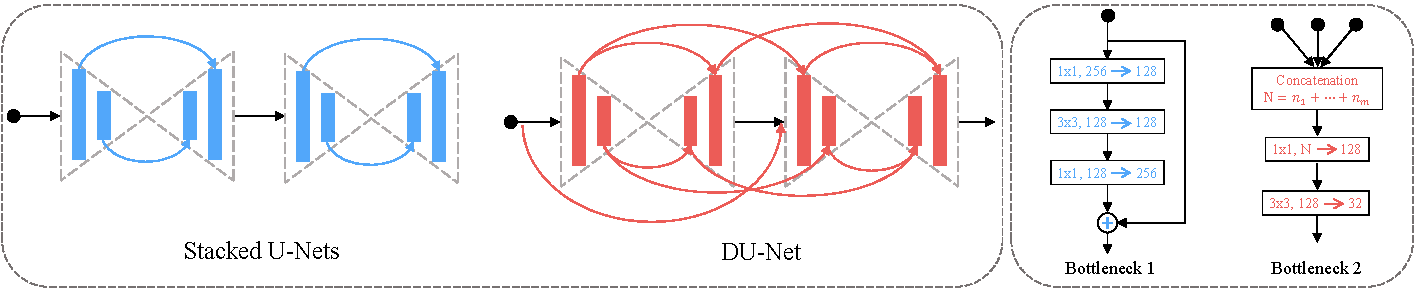
\includegraphics[width=1.0\linewidth]{figures/framework-cropped.pdf}
\caption{Illustration of stacked U-Nets and DU-Net. Stacked U-Nets has skip connections only within each U-Net. In contrast, DU-Net also connects blocks with the same semantic meanings across different U-Nets. The feature reuse could significantly reduce the size of bottleneck in each block, as shown in the right figure. Consequently, with the same number of U-Nets, DU-Net has only 30\% parameters of stacked U-Nets.}
\label{fig:framework}
\end{figure*}

% 
Our solution to those efficiency issues is threefold. {\bf First}, instead of connecting all stacked U-Nets, we only connect a U-Net to its $K$ successors. We name it as the $order$-$K$ connectivity, which aims to balance the fitting accuracy and parameter efficiency by cutting off long-distance connections. {\bf Second}, we employ a memory-efficient implementation in training. The key idea is to reuse a pre-allocated memory so all connected blocks could share the same memory. Compared with the naive implementation, this strategy makes it possible to train a very deep DU-Net (actually, $2\times$ deeper). {\bf Third}, to further improve the efficiency, we investigate an iterative design that may reduce the model size to one half. More specifically, the output of the first pass of the DU-Net is used as the input of the second pass, where detection or regression loss is applied as supervision. 

% %G%
% In view of deploying our approach on mobile devices, we further attempt to quantize weights, inputs, and gradients of DU-Net to low bit-width discrete values. This not only decreases the high precision operations but also shrinks the memory usage during training. By network quantization, the size of trained model can also be largely compressed.
% %G%
Besides shrinking the number of network parameters, we also study to further quantize each parameter. This motivates from the ubiquitous mobile applications. Although current mobile devices could carry models of dozens of MBs, deploying such networks requires high-end GPUs. However, quantized models could be accelerated by some specifically designed low-cost hardwares. Beyond only deploying models on mobile devices \cite{li2017deeprebirth}, training deep neural networks on distributed mobile devices emerges recently \cite{mcmahan2016communication}. To this end, we also try to quantize not only the model parameters but also its inputs (intermediate features) and gradients in training. This is the first attempt to investigate training landmark localizers using quantized inputs and gradients.


In summary, our key contributions are:
\begin{itemize}
    \item To the best of our knowledge, we are the first to propose quantized densely connected U-Nets for visual landmark localization, which largely improves the information flow and feature reuse at the semantic level.
    \item We propose the $order$-$K$ connectivity to balance accuracy and efficiency. It decreases the growth of model size from quadratic to linear by removing trivial connections. Experiments show it could reduce $\sim$70\% parameters of state-of-the-art landmark localizers.
    \item Very deep U-Nets can be trained using a memory-efficient implementation, where pre-allocated memory is reused by all connected blocks.
    \item We further investigate an iterative refinement that may cut down half of the model size, by forwarding DU-Net twice using either detection or regression supervision.
    %G%
    \item Different from previous efforts of quantizing only the model parameters, we are the first to quantize their inputs and gradients for better training efficiency on landmark localization tasks. By choosing appropriate quantization bit-widths for weights, inputs and gradients, quantized DU-Net achieves $\sim$75\% training memory saving with comparable performance. 
    %G%
    \item Exhaustive experiments are performed to validate DU-Net in different aspects. In both human pose estimation and face alignment, DU-Net demonstrates comparable localization accuracy and use $\sim$2\% model size compared with state-of-the-art methods.
\end{itemize}

% We are the first to deploy network quantization for better training efficiency on localization tasks. By choosing appropriate quantization bit-widths for weights, inputs and gradients, quantized DU-Net achieves at least 32$\times$ memory saving with comparable performance to the-state-of-art approaches. 


%The landmark localization such as human pose estimation \cite{toshev2014deeppose,newell2016stacked,wei2016convolutional}, facial landmark localization \cite{xiong2013supervised,zhang2014facial,sagonas2013300}, etc, plays an important role in the higher-level image understanding. The Convolutional Neural Networks (CNNs) have dominated this field, among which recent architecture of stacked hourglasses \cite{newell2016stacked}, a variant of the U-Net \cite{ronneberger2015unet}, becomes a standard solution. The skip connections between top-down and bottom-up blocks within a U-Net could preserve the spatial information and increase the gradient flow. With multiple U-Nets stacked together, the prediction could be refined stage by stage. However, the connections are only within each U-Net of the stacked hourglasses and no explicit connections exist between U-Nets, which may impede the information flow across them. And the blocks with the same semantics in different U-Nets cannot share features, leading to many redundant parameters. 

% Its success attributes to three key factors: repeated top-down, bottom-up inferences, intermediate supervisions and residual bottlenecks \cite{}. 

% The multiple stage top-down and bottom-up processing could better integrate both the local and global visual contexts into the final prediction. The intermediate supervision and residual bottlenecks, on the other hand, could alleviate the gradient vanish problem in deep networks.
%In this paper, we propose to densely connect stacked U-Nets by linking blocks with the same semantics in different U-Nets. We refer to this architecture as {\it Dense U-Nets}. The blocks in a U-Net could get direct inputs from its connected blocks in all preceding U-Nets, making the information flow more efficiently among the U-Nets. The feature reuse at each resolution could reduce the parameters in each block. The dense connectivity in our Dense U-Nets is different from that of DenseNet \cite{huang2016densely}. More specifically, layers only within each single block of the DenseNet are connected. In contrast, we connect blocks lying across the whole Dense U-Nets and connections of hierarchical blocks are mixed together. An illustration is given in Figure \ref{fig:framework}. We name it as the {\it global dense connectivity} to differentiate from the local one in the DenseNet.

% Besides, features in the Dense U-Nets are fused by the concatenation which could facilitate the information flow compared with the summation operation in the stacked hourglasses.

% Although the dense connectivity in our Dense U-Nets is similar with that of DenseNet \cite{}, 
% More recently, the DenseNet \cite{} achieves superior image classification performance over the ResNet \cite{} in terms of both the accuracy and model size, which benefits from the dense connections between layers. Its key insight is the feature reuse between layers of the same resolutions. The dense connectivity in the DenseNet, existing within one block, is local. By extending this principle, we propose a global dense connectivity, in contrast to the local connectivity in \cite{}, that blocks at the same locations of different U-Nets are connected. Hence, we refer to this architecture as {\it Dense U-Nets}. To our best knowledge, we are the first to generalize the local dense connectivity into the stacked U-Nets. 
% The global dense connectivity could make it easier to train much deeper stacked U-Nets.

% This motivates us to replace the residual modules  in the stacked hourglasses with the dense connected layers. However, this dense connectivity exists only locally within a contiguous  block in which all feature maps have the same spatial resolution. A U-Net, on the other hand, consists of a sequence of top-down and bottom-up blocks. A straight way is to turn each block into a dense block with multiple layers. However, this would sacrifice the spirit of stacked hourglasses that multiple stacked hourglasses outperform a single hourglass with multiple layers in each block.

% In order to integrate the structure of stacked U-Nets together with the idea of dense connectivity, we propose a global dense connectivity, in contrast to the local connectivity in \cite{}, that blocks at the same locations of different U-Nets are connected. Hence, we refer to this architecture as {\it Dense U-Nets}. The connected layers in the Dense U-Nets distribute along the whole network rather than in local continuous blocks. Compared with the local residual modules in the stacked hourglasses, the global dense connections could significantly facilitate the gradient to flow across stacked U-Nets.

%In practice, the Dense U-Nets have the efficiency problems of both parameter and training memory. First, suppose a Dense U-Nets contains $n$ U-Nets, there would be $O(n(n-1)/2)$ connections. Even though we use the dense bottleneck in Figure \ref{fig:framework}, the number of conv($1\times 1$) parameters still has the quadratic growth. Inspired from the Variable Order Markov (VOM) models \cite{begleiter2004prediction}, we propose the order-K connectivity that, instead of linking all the U-Nets, we connect only a fixed number of U-Nets. The goal is to use the minimum connections achieving the most obvious improvements. The multiple intermediate supervisions in the Dense U-Nets are good compensates for the order-K connectivity since they could provide additional gradients. The DenseNet does not have this advantage since it has only one supervision at the end.

% Furthermore, different from the DenseNet with only one supervision, the Dense U-Nets have multiple intermediate supervisions. The global dense connections plus the intermediate supervisions could bring faster convergence on the training set, but also gives rise to the concern of overfitting. Inspired from the Variable Order Markov (VOM) models \cite{}, we propose the order-K connectivity that, instead of linking all the U-Nets, we connect only a fixed number of U-Nets. The goal is to use the minimum connections achieving the most obvious improvement. Another advantage of order-K connectivity is that it has fewer parameters compared with the dense connectivity.

%Benefiting from the order-K connectivity, the Dense U-Nets could achieve comparable performance of stacked hourglasses with only one-third parameters. However, a naive implementation of the order-K connectivity could make the training very memory expensive. Therefore, we employ the memory efficient implementation \cite{pleiss2017memory}. The key idea is to share memories for time efficient operations such as concatenation and batch norm \cite{ioffe2015batch} within the connected layers. By pre-allocating a fixed memory, the later features produced by these operations would replace earlier features. So we need to re-compute those replaced features in the backward phase. The memory efficient implementation makes it possible to train Dense U-Nets two times deeper than the stacked hourglasses. 

%Furthermore, we also investigate to use the iterative refinement improving the parameter efficiency. Given a Dense U-Nets, we compare its performance with another Dense U-Nets with only half depth but an additional iteration. Besides, both detection and regression losses \cite{bulat2016human} were used in the landmark detection tasks, but there is no investigation yet about how they independently and collaboratively affect the prediction. We will give their detailed comparison in our experiments.

%In summary, the key contributions are:
%\begin{itemize}
%    \item To our best knowledge, we are the first to use the dense connectivity among the stacked U-Nets. The global dense connectivity in our Dense U-Nets is different from the local one in the DenseNet \cite{huang2016densely}.
%    \item We propose the order-K connectivity to make the Dense U-Nets parameter efficient. The order-K connectivity could decrease the growth of conv($1\times 1$) parameters from quadratic to linear. With comparable performance as the stacked hourglasses \cite{newell2016stacked}, it makes the Dense U-Nets require only one-third parameters. 
%    \item The memory efficient implementation of Dense U-Nets is provided to reduce its training memory usage. It makes it possible to train Dense U-Nets two times deeper than the stacked hourglasses.
%    \item We further explore using iterative refinement to improvement the parameter efficiency. At the same time, we investigate how different combinations of the detection and regression losses affect the performance.
%\end{itemize}
\section{Models}
\label{models}

So far we have motivated the need for better datasets and tasks to evaluate the
capabilities of machine reading models. We proceed by describing a number of
baselines, benchmarks and new models to evaluate against this paradigm.  We
define two simple baselines, the majority baseline ({\tt maximum frequency})
picks the entity most frequently observed in the context document, whereas the
exclusive majority ({\tt exclusive frequency}) chooses the entity most
frequently observed in the context but not observed in the query. The idea
behind this exclusion is that the placeholder is unlikely to be mentioned twice
in a single Cloze form query.

\subsection{Symbolic Matching Models}

Traditionally, a pipeline of NLP models has been used for attempting question
answering, that is models that make heavy use of linguistic annotation,
structured world knowledge and semantic parsing and similar NLP pipeline
outputs.
Building on these approaches, we define a number of NLP-centric models for our
machine reading task.

\paragraph{Frame-Semantic Parsing}

Frame-semantic parsing attempts to identify predicates and their arguments,
allowing models access to information about ``who did what to whom''. Naturally
this kind of annotation lends itself to being exploited for question answering.
We develop a benchmark that makes use of frame-semantic annotations
which we obtained by parsing our model with a state-of-the-art frame-semantic
parser \cite{Das:2013:SRL,Hermann:2014:SRL}. As the parser makes extensive use
of linguistic information we run these benchmarks on the unanonymised version of
our corpora. There is no significant advantage in this as the frame-semantic
approach used here does not possess the capability to generalise through a
language model beyond exploiting one during the parsing phase.
Thus, the key objective of evaluating machine comprehension abilities is
maintained. Extracting entity-predicate triples---denoted as
$(e_1,V,e_2)$---from both the query $q$ and context document $d$, we attempt to
resolve queries using a number of rules with an increasing recall/precision
trade-off as follows (Table \ref{tab:fsp}).

\begin{table}[h]\footnotesize
  \centering
  \begin{tabular}{@{}rllll@{}}
    \toprule
    & Strategy & Pattern $\in q$ & Pattern $\in d$ & Example (Cloze / Context) \\
    \midrule
    1 & Exact match & $(p,V,y)$ & $(\bm{x},V,y)$ & X loves Suse / \textbf{Kim} loves Suse \\
    2 & be.01.V match & $(p,\textit{be.01.V},y)$ & $(\bm{x},\textit{be.01.V},y)$ & X is president / \textbf{Mike} is president \\
    3 & Correct frame & $(p,V,y)$ & $(\bm{x},V,z)$ & X won Oscar / \textbf{Tom} won Academy Award \\
    4 & Permuted frame & $(p,V,y)$ & $(y,V,\bm{x})$ & X met Suse / Suse met \textbf{Tom} \\
    5 & Matching entity & $(p,V,y)$ & $(\bm{x},Z,y)$ & X likes candy / \textbf{Tom} loves candy \\
    6 & Back-off strategy & \multicolumn{3}{l}{\textit{Pick the most frequent entity from the context that doesn't appear in the query}} \\
    \bottomrule
  \end{tabular}
  \caption{Resolution strategies using PropBank triples. $\bm{x}$ denotes the
    entity proposed as answer, $V$ is a fully qualified PropBank frame (e.g.
    \textit{give.01.V}). Strategies are ordered by precedence and answers
    determined accordingly. This heuristic algorithm was iteratively
    tuned on the validation data set.
    \label{tab:fsp}
  }
\end{table}

For reasons of clarity, we pretend that all PropBank triples are of the form
$(e_1,V,e_2)$. In practice, we take the argument numberings of the parser into
account and only compare like with like, except in cases such as the permuted
frame rule, where ordering is relaxed. In the case of multiple possible answers
from a single rule, we randomly choose one.

\paragraph{Word Distance Benchmark}

We consider another baseline that relies on word distance measurements. Here, we
align the placeholder of the Cloze form question with each possible entity in
the context document and calculate a distance measure between the question and the
context around the aligned entity.
This score is calculated by summing the distances of every word in $q$
to their nearest aligned word in $d$, where alignment is defined by matching
words either directly or as aligned by the coreference system. We tune the
maximum penalty per word ($m=8$) on the validation data.

\subsection{Neural Network Models}
Neural networks have successfully been applied to a range of tasks in NLP.
This includes classification tasks such as sentiment analysis
\cite{Kalchbrenner:2014:DCNN} or POS tagging \cite{Collobert:2011:NLP}, as well
as generative problems such as language modelling or machine translation
\cite{Sutskever:2014:SSLNN}.
We propose three neural models for estimating the probability of word type $a$
from document $d$ answering query $q$:
\begin{align*}
  p(a | d, q) &\propto \exp \left(W(a) g(d,q) \right), \quad\text{s.t. } a \in
  V,
\end{align*}
where $V$ is the vocabulary\footnote{The vocabulary includes all the word types
  in the documents, questions, the entity maskers, and the question unknown
  entity marker.},
and $W(a)$ indexes row $a$ of weight matrix $W$ and through a slight abuse of
notation word types double as indexes. Note that we do not privilege entities or
variables, the model must learn to differentiate these in the input sequence.
The function $g(d,q)$ returns a vector embedding of a document and query pair.

\paragraph{The Deep LSTM Reader}
Long short-term memory (LSTM, \cite{Hochreiter:1997:LSTM}) networks have
recently seen considerable success in tasks such as machine translation and
language modelling \cite{Sutskever:2014:SSLNN}. When used for translation, Deep
LSTMs \cite{Graves:2012:SSLRNN} have shown a remarkable ability to embed long
sequences into a vector representation which contains enough information to
generate a full translation in another language. Our first neural model for
reading comprehension tests the ability of Deep LSTM encoders to handle
significantly longer sequences. We feed our documents one word at a time into
a Deep LSTM encoder, after a delimiter we then also feed the query into the
encoder. Alternatively we also experiment with processing the query then the
document. The result is that this model processes each document query pair as a
single long sequence. Given the embedded document and query the network
predicts which token in the document answers the query.

We employ a Deep LSTM cell with skip connections from each input $x(t)$ to every
hidden layer, and from every hidden layer to the output $y(t)$:
\begin{align*}
  x'(t,k) &= x(t)||y'(t,k-1), \quad\quad y(t) = y'(t,1) || \ldots || y'(t,K) \\
  \igate(t,k) &= \sigma\left(\wtmat{kx}{\igate} x'(t,k) + \wtmat{kh}{\igate} h(t-1,k) + \wtmat{k\state}{\igate} \state(t-1,k)  + b_{k\igate}\right)\\
  \fgate(t,k) &= \sigma\left(\wtmat{kx}{\fgate} x(t) + \wtmat{kh}{\fgate} h(t-1,k) + \wtmat{k\state}{\fgate} \state(t-1,k) + b_{k\fgate} \right)\\
  \state(t,k) &= \fgate(t,k) \state(t-1,k) + \igate(t,k) \tanh \left(\wtmat{kx}{\state} x'(t,k) + \wtmat{kh}{\state} h(t-1,k) + b_{k\state} \right) \\
  \ogate(t,k) &= \sigma\left(\wtmat{kx}{\ogate} x'(t,k) + \wtmat{kh}{\ogate} h(t-1,k) + \wtmat{k\state}{\ogate} \state(t,k) + b_{k\ogate}\right)\\
  h(t,k) &= \ogate(t,k) \tanh\left(\state(t,k)\right)\\
  y'(t,k) &= \wtmat{k}{y}h(t,k) + b_{ky}
\end{align*}
where $||$ indicates vector concatenation $h(t,k)$ is the hidden state for layer
$k$ at time $t$, and $\igate$, $\fgate$, $\ogate$ are the input, forget, and
output gates respectively.
Thus our Deep LSTM Reader is defined by $g^{\text{\tiny LSTM}}(d,q) = y(|d|+|q|)$ with input $x(t)$ the concatenation of $d$ and $q$ separated by the delimiter $|||$.

\paragraph{The Attentive Reader}

\newcommand{\attnIn}{m}
\newcommand{\attnU}{u}
\newcommand{\attnOver}{y}
\newcommand{\attnMix}{r}
\newcommand{\attnMid}{z}
\newcommand{\attnScore}{s}
\newcommand{\fwd}[1]{\overrightarrow{#1}}
\newcommand{\back}[1]{\overleftarrow{#1}}
\newcommand{\softmax}[2]{\frac{\exp\left(#1\right)}{#2}}

\begin{figure}
\centering
  \begin{subfigure}[b]{0.49\textwidth}
    \centering
    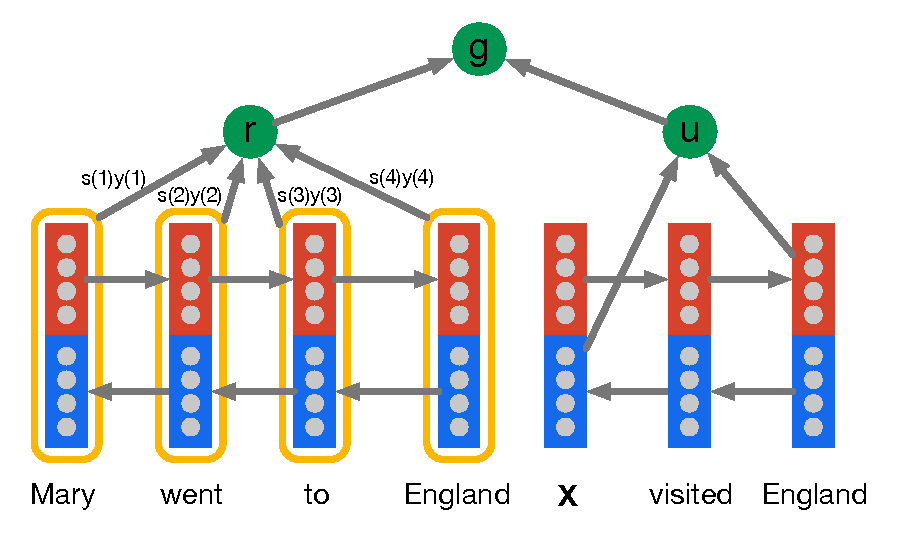
\includegraphics[scale=0.44]{figs/AttentiveReader.pdf}
    \caption{Attentive Reader.}
  \end{subfigure}
  \begin{subfigure}[b]{0.49\textwidth}
    \centering
    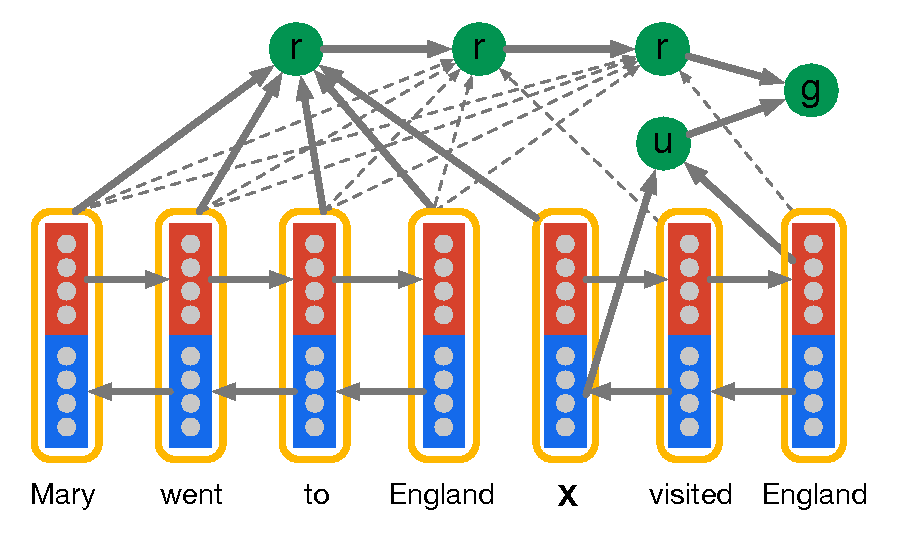
\includegraphics[scale=0.44]{figs/ImpatientReader.pdf}
    \caption{Impatient Reader.}
  \end{subfigure}
  \begin{subfigure}[b]{1.0\textwidth}
    \centering
    %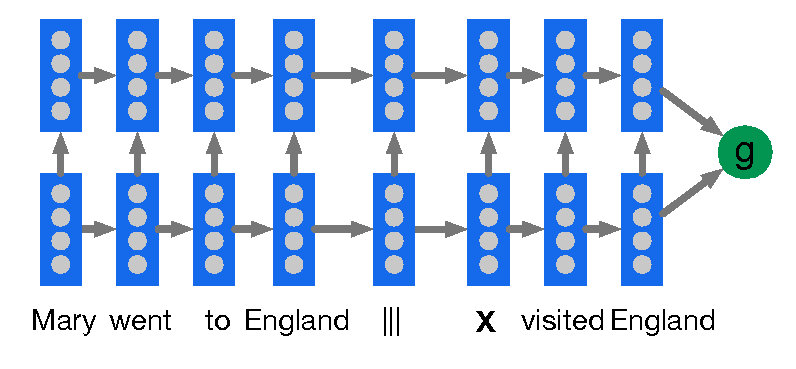
\includegraphics[scale=0.40]{figs/BiLSTM.pdf}
    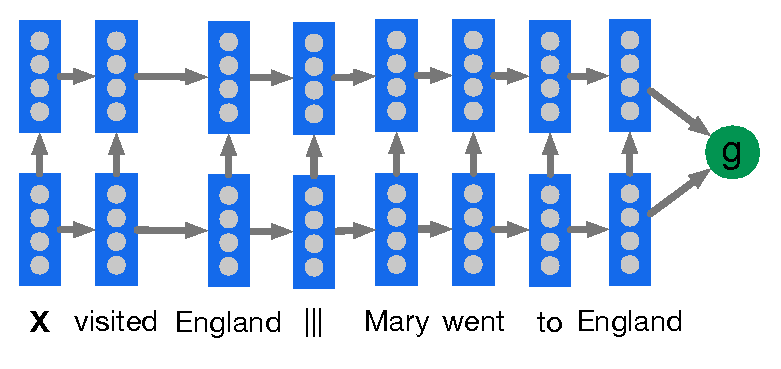
\includegraphics[scale=0.44]{figs/BiLSTMRev.pdf}
    \caption{A two layer Deep LSTM Reader with the question encoded before
             the document.}
  \end{subfigure}
  \caption{Document and query embedding models.}
\label{fig:models}
\end{figure}

The Deep LSTM Reader must propagate dependencies over long distances in order to
connect queries to their answers. The fixed width hidden vector forms a
bottleneck for this information flow that we propose to circumvent using an
attention mechanism inspired by recent results in translation and image
recognition \cite{Bahdanau:2014:NMT,Mnih:2014:RMVA}.
This attention model first encodes the document and the query using separate
bidirectional single layer LSTMs \cite{Graves:2012:SSLRNN}.

We denote the
outputs of the forward and backward LSTMs as $\fwd{y}(t)$ and $\back{y}(t)$
respectively.  The encoding $u$ of a query of length $|q|$ is formed by the
concatenation of the final forward and backward outputs,
$u = \fwd{y_q}(|q|)\,\, ||\,\, \back{y_q}(1).$

For the document the composite output for each token at position $t$ is,
$y_d(t) = \fwd{y_d}(t)\,\, ||\,\, \back{y_d}(t).$
The representation $r$ of the document $d$ is formed by a weighted sum of these
output vectors. These weights are interpreted as the degree to which the network
attends to a particular token in the document when answering the query:
\begin{align*}
  \attnIn(t)    &= \tanh\left(\wtmat{\attnOver}{\attnIn} \attnOver_d(t)
                   + \wtmat{\attnU}{\attnIn} \attnU\right),\\
  \attnScore(t) &\propto \exp \left(\mathrm{w}_{\attnIn\attnScore}^\intercal
                         \attnIn(t) \right),\\
  \attnMix   &= \attnOver_d \attnScore,
\end{align*}
where we are interpreting $y_d$ as a matrix with each column being the composite
representation $y_d(t)$ of document token $t$.
The variable $\attnScore(t)$ is the normalised attention at token $t$. Given
this attention score the embedding of the document $\attnMix$ is computed as the
weighted sum of the token embeddings.
The model is completed with the definition of the joint document and query
embedding via a non-linear combination:
\begin{align*}
  g^{\text{\tiny AR}}(d,q) = \tanh \left(\wtmat{\attnMix}{g} \attnMix
                             + \wtmat{\attnU}{g} \attnU \right).
\end{align*}

The Attentive Reader can be viewed as a generalisation of the application of
Memory Networks to question answering \cite{Weston:2014:MN}. That model employs
an attention mechanism at the sentence level where each sentence is represented
by a bag of embeddings. The Attentive Reader employs a finer grained token
level attention mechanism where the tokens are embedded given their entire
future and past context in the input document.

\paragraph{The Impatient Reader}
The Attentive Reader is able to focus on the passages of a context document
that are most likely to inform the answer to the query. We can go further by
equipping the model with the ability to reread from the document as each query
token is read. At each token $i$ of the query $q$ the model computes a document
representation vector $r(i)$ using the bidirectional embedding $y_q(i) =
\fwd{y_q}(i)\,\, ||\,\, \back{y_q}(i)$:
\begin{align*}
  \attnIn(i, t)   &= \tanh\left(\wtmat{d}{\attnIn} \attnOver_d(t)
                   + \wtmat{\attnMix}{\attnIn} \attnMix(i-1)
                   + \wtmat{q}{\attnIn} y_q(i) \right)
                , \quad 1 \leq i \leq |q|,  \\
  \attnScore(i,t) &\propto \exp \left(\mathrm{w}_{\attnIn\attnScore}^\intercal
                   \attnIn(i,t) \right),\\
  \attnMix(0)     &= \mathbf{r_0}, \quad
                   \attnMix(i)     = \attnOver_d^\intercal \attnScore(i) +
                   \tanh\left(\wtmat{\attnMix}{\attnMix}\attnMix(i-1)\right)
  \quad 1 \leq i \leq |q|.
\end{align*}
The result is an attention mechanism that allows the model to recurrently
accumulate information from the document as it sees each query token, ultimately
outputting a final joint document query representation for the answer prediction,
\begin{align*}
  g^{\text{\tiny IR}}(d,q) = \tanh \left(\wtmat{\attnMix}{g} \attnMix(|q|) +
                             \wtmat{q}{g} \attnU \right).
\end{align*}

The majority of existing approaches to WSD formulate this task as  MIL. In this formulation an image is interpreted as a bag of regions. If the image is labeled as positive, then one of the regions is assume to tightly contain the object of interest. If the image is labeled as negative, then no region contains the object. Learning alternates between estimating a model of the object appearance and selecting which regions in the positive bags correspond to the object using the appearance model. 

The MIL strategy results in a non-convex optimization problem; in practice, solvers tend to get stuck in local optima such that the quality of the solution strongly depends on the initialization. Several papers have focused on developing various initialization strategies \cite{Kumar10a,Deselaers10,Song14a,Cinbis15} and on regularizing the optimization problem \cite{Song14,Bilen14}. Kumar~\etal \cite{Kumar10a} propose a self-paced learning strategy that progressively includes harder samples to a small set of initial ones at training. Deselaers~\etal~\cite{Deselaers10} initialize object locations based on the objectness score. Cinbis~\etal \cite{Cinbis15} propose a multi-fold split of the training data to escape local optima. Song~\etal~\cite{Song14} apply Nesterov's smoothing technique \cite{Nesterov05} to the latent SVM formulation \cite{Felzenszwalb10a} to be more robust against poor initializations. Bilen~\etal~\cite{Bilen14} propose a smoothed version of MIL that softly labels object instances instead of choosing the highest scoring ones. Additionally, their method regularizes the latent object locations by penalizing unlikely configurations based on symmetry and mutual exclusion principles.

Another line of research in WSD \cite{Song14,Song14a,Wang14a} is based on the idea of identifying the similarity between image parts. Song~\etal \cite{Song14} propose a discriminative graph-based algorithm that selects a subset of windows such that each window is connected to its nearest neighbors in positive images. In~\cite{Song14a}, the same authors extend this method to discover multiple co-occurring part configurations. Wang~\etal~\cite{Wang14a} propose an iterative technique that applies a latent semantic clustering via latent Semantic Analysis (pLSA) on the windows of positive samples and selects the most discriminative cluster for each class based on its classification performance. Bilen~\etal \cite{Bilen15} propose a formulation that jointly learns a discriminative model and enforces the similarity of the selected object regions via a discriminative convex clustering algorithm.

Recently a number of researchers \cite{Oquab14,Oquab15} have proposed weakly supervised localization principles to improve classification performance of CNNs without providing any annotation for the location of objects in images. Oquab~\etal \cite{Oquab14} employ a pre-trained CNN to compute a mid-level image representation for images of PASCAL VOC. In their follow-up work, Oquab~\etal \cite{Oquab15} modify a CNN architecture to \emph{coarsely} localize object instances in image while predicting its label. 

Jaderberg~\etal~\cite{Jaderberg15c} proposed a CNN architecture in which a subnetwork automatically pre-transforms an image in order to optimize the classification accuracy of a second subnetwork. This ``transformer network'', which is trained in an end-to-end fashion from image-level labels, is shown to align objects to a common reference frame, which is a proxy to detection. Our architecture contains a mechanism that pre-select image regions that are likely to contain the object, also trained in an end-to-end fashion; while this may seem very different, this mechanism can also be thought as learning transformations (as the ones that map the detected regions to a canonical reference frame). However, the nature of the selection process in in our and their networks are very different.

\section{Experiments}
\label{sect:experiments}

% \begin{figure*}
%   \centering
%   \setlength{\tabcolsep}{0pt}
%   \setlength\figurewidth{0.05\textwidth}
%   \newcommand{\example}[1]{\raisebox{-.4\height}{\includegraphics[width=\figurewidth]{./figures/domains_examples/#1}}}
%   \begin{sc}
%   \begin{tabular}{r@{\hskip 1cm} ccccccccccc}
%     MNIST \cite{LeCun98} &
%     \example{mnist_0.png} &
%     \example{mnist_1.png} &
%     \example{mnist_2.png} &
%     \example{mnist_3.png} &
%     \example{mnist_4.png} &
%     \example{mnist_5.png} &
%     \example{mnist_6.png} &
%     \example{mnist_7.png} &
%     \example{mnist_8.png} &
%     \example{mnist_9.png} &
%     \example{mnist_10.png}\\
%     MNIST ($ | \Delta | $, BG) &
%     \example{mnisti_0.png} &
%     \example{mnisti_1.png} &
%     \example{mnisti_2.png} &
%     \example{mnisti_3.png} &
%     \example{mnisti_4.png} &
%     \example{mnisti_5.png} &
%     \example{mnisti_6.png} &
%     \example{mnisti_7.png} &
%     \example{mnisti_8.png} &
%     \example{mnisti_9.png} &
%     \example{mnisti_10.png}\\
%     Syn Numbers &
%     \example{syn_0.png} &
%     \example{syn_1.png} &
%     \example{syn_2.png} &
%     \example{syn_3.png} &
%     \example{syn_4.png} &
%     \example{syn_5.png} &
%     \example{syn_6.png} &
%     \example{syn_7.png} &
%     \example{syn_8.png} &
%     \example{syn_9.png} &
%     \example{syn_10.png}\\
%     SVHN \cite{Netzer11} &
%     \example{svhn_0.png} &
%     \example{svhn_1.png} &
%     \example{svhn_2.png} &
%     \example{svhn_3.png} &
%     \example{svhn_4.png} &
%     \example{svhn_5.png} &
%     \example{svhn_6.png} &
%     \example{svhn_7.png} &
%     \example{svhn_8.png} &
%     \example{svhn_9.png} &
%     \example{svhn_10.png}\\
%     Syn Signs &
%     \example{synsgn_11.png} &
%     \example{synsgn_1.png} &
%     \example{synsgn_2.png} &
%     \example{synsgn_3.png} &
%     \example{synsgn_4.png} &
%     \example{synsgn_5.png} &
%     \example{synsgn_12.png} &
%     \example{synsgn_7.png} &
%     \example{synsgn_8.png} &
%     \example{synsgn_9.png} &
%     \example{synsgn_10.png}\\
%     GTSRB \cite{Stallkamp12} &
%     \example{gtsrb_0.png} &
%     \example{gtsrb_1.png} &
%     \example{gtsrb_2.png} &
%     \example{gtsrb_3.png} &
%     \example{gtsrb_4.png} &
%     \example{gtsrb_5.png} &
%     \example{gtsrb_6.png} &
%     \example{gtsrb_7.png} &
%     \example{gtsrb_8.png} &
%     \example{gtsrb_9.png} &
%     \example{gtsrb_10.png}\\
%     % CIFAR-10 \cite{Krizhevsky09} &
%     % \example{cifar10_0.png} &
%     % \example{cifar10_1.png} &
%     % \example{cifar10_2.png} &
%     % \example{cifar10_3.png} &
%     % \example{cifar10_4.png} &
%     % \example{cifar10_5.png} &
%     % \example{cifar10_11.png} &
%     % \example{cifar10_7.png} &
%     % \example{cifar10_8.png} &
%     % \example{cifar10_9.png} &
%     % \example{cifar10_10.png}\\
%     % STL-10 \cite{Coates11} &
%     % \example{stl10_12.png} &
%     % \example{stl10_1.png} &
%     % \example{stl10_2.png} &
%     % \example{stl10_3.png} &
%     % \example{stl10_4.png} &
%     % \example{stl10_5.png} &
%     % \example{stl10_6.png} &
%     % \example{stl10_13.png} &
%     % \example{stl10_8.png} &
%     % \example{stl10_9.png} &
%     % \example{stl10_10.png}\\
%   \end{tabular}
%   \end{sc}
%   \vskip 2.5mm
%   \caption{\todo[What to do with this figure? Add Office? Remove?]Random samples from the datasets used in the experiments. See \sect{exper_quant} for details.}
%   \label{fig:exper_domains_examples}
% \end{figure*}

\begin{figure*}
  \centering
  \setlength{\tabcolsep}{0pt}
  \setlength\figurewidth{0.05\textwidth}
  \newcommand{\example}[1]{\raisebox{-.4\height}{\includegraphics[width=\figurewidth]{./figures/domains_examples/#1}}}
  \begin{sc}
  \begin{small}
  \begin{tabular}{r@{\hskip 0.5cm} ccc c@{\hskip 0.4cm} ccc c@{\hskip 0.4cm} ccc c@{\hskip 0.4cm} ccc}
    &
    \multicolumn{3}{c}{MNIST} & &
    \multicolumn{3}{c}{Syn Numbers} & &
    \multicolumn{3}{c}{SVHN} & &
    \multicolumn{3}{c}{Syn Signs}\\
    
    Source &
    \example{mnist_0.png} &
    \example{mnist_1.png} &
    \example{mnist_3.png} & &
    
    \example{syn_0.png} &
    \example{syn_1.png} &
    \example{syn_2.png} & &
    
    \example{svhn_3.png} &
    \example{svhn_4.png} &
    \example{svhn_5.png} & &
    
    \example{synsgn_3.png} &
    \example{synsgn_4.png} &
    \example{synsgn_5.png}\\
    
    Target &
    \example{mnisti_0.png} &
    \example{mnisti_1.png} &
    \example{mnisti_2.png} & &
    
    \example{svhn_0.png} &
    \example{svhn_1.png} &
    \example{svhn_2.png} & &
    
    \example{mnist_4.png} &
    \example{mnist_5.png} &
    \example{mnist_6.png} & &
    
    \example{gtsrb_2.png} &
    \example{gtsrb_3.png} &
    \example{gtsrb_4.png}\\
    
    &
    \multicolumn{3}{c}{\rule{0pt}{0.35cm} MNIST-M} & &
    \multicolumn{3}{c}{SVHN} & &
    \multicolumn{3}{c}{MNIST} & &
    \multicolumn{3}{c}{GTSRB}\\
  \end{tabular}
  \end{small}
  \end{sc}
  \caption{Examples of domain pairs used in the experiments. See \sect{exper_quant} for details.}
  \label{fig:exper_domains_examples}
\end{figure*}


\begin{table*}[t]
  \vskip 0.15in
  \begin{center}
    \begin{small}
      \begin{sc}
        \renewcommand{\arraystretch}{1.5}
        \begin{tabular}{l r | c c c c}
          \hline
          \multirow{2}{*}{Method} & {\scriptsize Source} & MNIST & Syn Numbers & SVHN & Syn Signs \\
          & {\scriptsize Target} & MNIST-M & SVHN & MNIST & GTSRB \\
          \hline
          \multicolumn{2}{l |}{Source only} & 
          $ .5749 $                      & $ .8665 $                      & $ .5919 $                      & $ .7400 $                      \\
          \multicolumn{2}{l |}{SA \cite{Fernando13}} & 
          $ .6078 \; (7.9\%) $           & $ .8672 \; (1.3\%) $           & $ .6157 \; (5.9\%) $           & $ .7635 \; (9.1\%) $           \\
          \multicolumn{2}{l |}{Proposed approach} & 
          $ \mathbf{.8149} \; (57.9\%) $ & $ \mathbf{.9048} \; (66.1\%) $ & $ \mathbf{.7107} \; (29.3\%) $ & $ \mathbf{.8866} \; (56.7\%) $ \\
          \multicolumn{2}{l |}{Train on target} & 
          $ .9891 $                      & $ .9244 $                      & $ .9951 $                      & $ .9987 $                      \\
          \hline
        \end{tabular}
      \end{sc}
    \end{small}
  \end{center}
    \caption{Classification accuracies for digit image classifications for different source and target domains. {\sc MNIST-M} corresponds to difference-blended digits over non-uniform background. The first row corresponds to the lower performance bound (i.e.\ if no adaptation is performed). The last row corresponds to training on the target domain data with known class labels (upper bound on the DA performance). For each of the two DA methods (ours and \cite{Fernando13}) we show how much of the gap between the lower and the upper bounds was covered (in brackets). For all five cases, our approach outperforms \cite{Fernando13} considerably, and covers a big portion of the gap.\vspace{-0mm} }
  \label{tab:results}
  \vskip -0.1in
\end{table*}

\begin{table*}[t]
  \vskip 0.15in
  \begin{center}
    \begin{small}
      \begin{sc}
        \renewcommand{\arraystretch}{1.5}
        \begin{tabular}{l r | c c c}
          \hline
          \multirow{2}{*}{Method} & {\scriptsize Source} & Amazon & DSLR & Webcam \\
          & {\scriptsize Target} & Webcam & Webcam & DSLR \\
          \hline
          \multicolumn{2}{l |}{GFK(PLS, PCA) \cite{Gong12}} & 
          $ .464 \pm .005 $ & $ .613 \pm .004 $ & $ .663 \pm .004 $\\ 
          \multicolumn{2}{l |}{SA \cite{Fernando13}} & 
          $ .450 $ & $ .648 $ & $ .699 $\\ 
          \multicolumn{2}{l |}{DA-NBNN \cite{Tommasi13}} & 
          $ .528 \pm .037 $ & $ .766 \pm .017 $ & $ .762 \pm .025 $\\ 
          \multicolumn{2}{l |}{DLID \cite{Chopra13}} & 
          $ .519 $ & $ .782 $ & $ .899 $\\
          \multicolumn{2}{l |}{DeCAF$_6$ Source Only \cite{Donahue14}} &
          $ .522 \pm .017 $ & $ .915 \pm .015 $ & --\\ 
          \multicolumn{2}{l |}{DaNN \cite{Ghifary14}} & 
          $ .536 \pm .002 $ & $ .712 \pm .000 $ & $ .835 \pm .000 $\\ 
          \multicolumn{2}{l |}{DDC \cite{Tzeng14}} & 
          $ .594 \pm .008 $ & $ .925 \pm .003 $ & $ .917 \pm .008 $\\ 
          \multicolumn{2}{l |}{Proposed Approach} & 
          $ \mathbf{ .673 \pm .017 } $ & $ \mathbf{ .940 \pm .008 } $ & $ \mathbf{ .937 \pm .010 } $\\
          \hline
        \end{tabular}
      \end{sc}
    \end{small}
  \end{center}
    \caption{Accuracy evaluation of different DA approaches on the standard {\sc Office} \cite{Saenko10} dataset. Our method (last row) outperforms competitors setting the new state-of-the-art.}
  \label{tab:results_office}
\end{table*}

% Other rows refer to the following algorithms (from top to bottom): Geodesic Flow Kernel \cite{Gong12}, Subspace Alignment \cite{Fernando13}, Naive Bayes Nearest Neighbor \cite{Tommasi13},  deep learning approach from \cite{Chopra13}, DeCAF$_6$-features described in \cite{Donahue14}, Domain Adaptive NNs \cite{Ghifary14}, Deep Domain Confusion \cite{Tzeng14}.

\def\X{{\mathbf X}}
\def\y{{\mathbf y}}

% \vspace{2mm}\noindent {\bf Datasets.}
% \label{sect:exper_datasets}

% In order to test our method in the setting of traffic signs classification we obtained~100,000 synthetic images ({\sc Syn~Signs}) simulating various photoshooting conditions. This dataset was used in conjunction with {\it The German Traffic Sign Recognition Benchmark} ({\sc GTSRB}) \cite{Stallkamp12}.

% Finally, we perform domain adaption for the {\sc CIFAR-10} and the {\sc STL-10} downsampled to the size of $ 32 \times 32 $. This pair is considerably different from the previously mentioned datasets as the intra-class variability here is higher.

We perform extensive evaluation of the proposed approach on a number of popular image datasets and their modifications. These include large-scale datasets of small images popular with deep learning methods, and the {\sc Office} datasets \cite{Saenko10}, which are a {\em de facto} standard for domain adaptation in computer vision, but have much fewer images.

\vspace{2mm}\noindent {\bf Baselines.} For the bulk of experiments the following baselines are evaluated. The \textbf{source-only} model is trained without consideration for target-domain data (no domain classifier branch included into the network). The \textbf{train-on-target} model is trained on the target domain with class labels revealed. This model serves as an upper bound on DA methods, assuming that target data are abundant and the shift between the domains is considerable. 

In addition, we compare our approach against the recently proposed unsupervised DA method based on \textbf{subspace alignment (SA)} \cite{Fernando13}, which is simple to setup and test on new datasets, but has also been shown to perform very well in experimental comparisons with other ``shallow'' DA methods. To boost the performance of this baseline, we pick its most important free parameter (the number of principal components) from the range $ \{ 2, \ldots, 60 \} $, so that the test performance on the target domain is maximized. To apply SA in our setting, we train a source-only model and then consider the activations of the last hidden layer in the label predictor (before the final linear classifier) as descriptors/features, and learn the mapping between the source and the target domains \cite{Fernando13}.

Since the SA baseline requires to train a new classifier after adapting the features, and in order to put all the compared settings on an equal footing, we retrain the last layer of the label predictor using a standard linear SVM~\cite{liblinear} for all four considered methods (including ours; the performance on the target domain remains approximately the same after the retraining). 

For the {\sc Office} dataset \cite{Saenko10}, we directly compare the performance of our full network (feature extractor and label predictor) against recent DA approaches using previously published results.

\vspace{2mm}\noindent {\bf CNN architectures.} In general, we compose feature extractor from two or three convolutional layers, picking their exact configurations from previous works. We give the exact architectures in \ref{sect:appendix_archs}.

For the domain adaptator we stick to the three fully connected layers ($x\rightarrow1024\rightarrow1024\rightarrow2$), except for {\sc MNIST} where we used a simpler ($x\rightarrow100\rightarrow2$) architecture to speed up the experiments.

For loss functions, we set $ L_y $ and $ L_d $ to be the logistic regression loss and the binomial cross-entropy respectively.

\vspace{2mm}\noindent {\bf CNN training procedure.}
The model is trained on $128$-sized batches. Images are preprocessed by the mean subtraction. A half of each batch is populated by the samples from the source domain (with known labels), the rest is comprised of the target domain (with unknown labels).

In order to suppress noisy signal from the domain classifier at the early stages of the training procedure instead of fixing the adaptation factor $ \lambda $, we gradually change it from $0$ to $1$ using the following schedule:
\begin{equation}
  \lambda_p = \frac{2}{1 + \exp(-\gamma \cdot p)} - 1,
\end{equation}
where $\gamma$ was set to $10$ in all experiments (the schedule was not optimized/tweaked). Further details on the CNN training can be found in \ref{sect:appendix_training}.

\vspace{2mm}\noindent {\bf Visualizations.}
We use t-SNE \cite{Maaten13} projection to visualize feature distributions at different points of the network, while color-coding the domains (\fig{exper_adapt_vis}). We observe strong correspondence between the success of the adaptation in terms of the classification accuracy for the target domain, and the overlap between the domain distributions in such visualizations.
 
\vspace{2mm}\noindent {\bf Choosing meta-parameters.} 
In general, good unsupervised DA methods should provide ways to set meta-parameters (such as $\lambda$, the learning rate, the momentum rate, the network architecture for our method) in an unsupervised way, i.e.\ without referring to labeled data in the target domain. %Here we would like to give few recommendations concerning this matter. First, as it was pointed out in \sect{theory} the domain classifier should not be significantly more complex than the label predictor. 
In our method, one can assess the performance of the whole system (and the effect of changing hyper-parameters) by observing the test error on the source domain {\em and} the domain classifier error. In general, we observed a good correspondence between the success of adaptation and these errors (adaptation is more successful when the source domain test error is low, while the domain classifier error is high).
In addition, the layer, where the the domain adaptator is attached can be picked by computing difference between means as suggested in \cite{Tzeng14}. 

% \begin{figure*}
%   \centering
%   {\sc MNIST $ \rightarrow $ MNIST ($ | \Delta | $, bg)}: top feature extractor layer
%   \setcounter{subfigure}{0}
%   \subfigure[Non-adapted]{%%
%     \scalebox{0.8}{%% Creator: Matplotlib, PGF backend
%%
%% To include the figure in your LaTeX document, write
%%   \input{<filename>.pgf}
%%
%% Make sure the required packages are loaded in your preamble
%%   \usepackage{pgf}
%%
%% Figures using additional raster images can only be included by \input if
%% they are in the same directory as the main LaTeX file. For loading figures
%% from other directories you can use the `import` package
%%   \usepackage{import}
%% and then include the figures with
%%   \import{<path to file>}{<filename>.pgf}
%%
%% Matplotlib used the following preamble
%%   \usepackage[utf8x]{inputenc}
%%   \usepackage[T1]{fontenc}
%%
\begingroup%
\makeatletter%
\begin{pgfpicture}%
\pgfpathrectangle{\pgfpointorigin}{\pgfqpoint{3.338520in}{2.040000in}}%
\pgfusepath{use as bounding box}%
\begin{pgfscope}%
\pgfsetbuttcap%
\pgfsetroundjoin%
\definecolor{currentfill}{rgb}{1.000000,1.000000,1.000000}%
\pgfsetfillcolor{currentfill}%
\pgfsetlinewidth{0.000000pt}%
\definecolor{currentstroke}{rgb}{1.000000,1.000000,1.000000}%
\pgfsetstrokecolor{currentstroke}%
\pgfsetdash{}{0pt}%
\pgfpathmoveto{\pgfqpoint{0.000000in}{-0.000000in}}%
\pgfpathlineto{\pgfqpoint{3.338520in}{-0.000000in}}%
\pgfpathlineto{\pgfqpoint{3.338520in}{2.040000in}}%
\pgfpathlineto{\pgfqpoint{0.000000in}{2.040000in}}%
\pgfpathclose%
\pgfusepath{fill}%
\end{pgfscope}%
\begin{pgfscope}%
\pgftext[at=\pgfqpoint{0.510000in}{0.348333in},left,bottom]{\pgfimage[interpolate=true,width=2.553333in,height=1.500000in]{./figures/adaptation_vis/pool2_mnist2inv_before-img0.png}}%
\end{pgfscope}%
\begin{pgfscope}%
\pgftext[at=\pgfqpoint{0.805000in}{0.383333in},left,bottom]{\pgfimage[interpolate=true,width=2.201667in,height=1.371667in]{./figures/adaptation_vis/pool2_mnist2inv_before-img1.png}}%
\end{pgfscope}%
\end{pgfpicture}%
\makeatother%
\endgroup%
}}%%
%   \subfigure[Adapted]{%%
%     \scalebox{0.8}{%% Creator: Matplotlib, PGF backend
%%
%% To include the figure in your LaTeX document, write
%%   \input{<filename>.pgf}
%%
%% Make sure the required packages are loaded in your preamble
%%   \usepackage{pgf}
%%
%% Figures using additional raster images can only be included by \input if
%% they are in the same directory as the main LaTeX file. For loading figures
%% from other directories you can use the `import` package
%%   \usepackage{import}
%% and then include the figures with
%%   \import{<path to file>}{<filename>.pgf}
%%
%% Matplotlib used the following preamble
%%   \usepackage[utf8x]{inputenc}
%%   \usepackage[T1]{fontenc}
%%
\begingroup%
\makeatletter%
\begin{pgfpicture}%
\pgfpathrectangle{\pgfpointorigin}{\pgfqpoint{3.340000in}{2.040000in}}%
\pgfusepath{use as bounding box}%
\begin{pgfscope}%
\pgfsetbuttcap%
\pgfsetroundjoin%
\definecolor{currentfill}{rgb}{1.000000,1.000000,1.000000}%
\pgfsetfillcolor{currentfill}%
\pgfsetlinewidth{0.000000pt}%
\definecolor{currentstroke}{rgb}{1.000000,1.000000,1.000000}%
\pgfsetstrokecolor{currentstroke}%
\pgfsetdash{}{0pt}%
\pgfpathmoveto{\pgfqpoint{0.000000in}{-0.000000in}}%
\pgfpathlineto{\pgfqpoint{3.340000in}{-0.000000in}}%
\pgfpathlineto{\pgfqpoint{3.340000in}{2.040000in}}%
\pgfpathlineto{\pgfqpoint{0.000000in}{2.040000in}}%
\pgfpathclose%
\pgfusepath{fill}%
\end{pgfscope}%
\begin{pgfscope}%
\pgftext[at=\pgfqpoint{0.518333in}{0.321667in},left,bottom]{\pgfimage[interpolate=true,width=2.565000in,height=1.550000in]{./figures/adaptation_vis/pool2_mnist2inv_after-img0.png}}%
\end{pgfscope}%
\begin{pgfscope}%
\pgftext[at=\pgfqpoint{0.518333in}{0.321667in},left,bottom]{\pgfimage[interpolate=true,width=2.565000in,height=1.553333in]{./figures/adaptation_vis/pool2_mnist2inv_after-img1.png}}%
\end{pgfscope}%
\end{pgfpicture}%
\makeatother%
\endgroup%
}}\\
%   \vspace{5mm}
%   {\sc Syn Numbers $ \rightarrow $ SVHN}: last hidden layer of the label predictor
%   \setcounter{subfigure}{0}
%   \subfigure[Non-adapted]{%%
%     \scalebox{0.8}{%% Creator: Matplotlib, PGF backend
%%
%% To include the figure in your LaTeX document, write
%%   \input{<filename>.pgf}
%%
%% Make sure the required packages are loaded in your preamble
%%   \usepackage{pgf}
%%
%% Figures using additional raster images can only be included by \input if
%% they are in the same directory as the main LaTeX file. For loading figures
%% from other directories you can use the `import` package
%%   \usepackage{import}
%% and then include the figures with
%%   \import{<path to file>}{<filename>.pgf}
%%
%% Matplotlib used the following preamble
%%   \usepackage[utf8x]{inputenc}
%%   \usepackage[T1]{fontenc}
%%
\begingroup%
\makeatletter%
\begin{pgfpicture}%
\pgfpathrectangle{\pgfpointorigin}{\pgfqpoint{3.340000in}{2.040000in}}%
\pgfusepath{use as bounding box}%
\begin{pgfscope}%
\pgfsetbuttcap%
\pgfsetroundjoin%
\definecolor{currentfill}{rgb}{1.000000,1.000000,1.000000}%
\pgfsetfillcolor{currentfill}%
\pgfsetlinewidth{0.000000pt}%
\definecolor{currentstroke}{rgb}{1.000000,1.000000,1.000000}%
\pgfsetstrokecolor{currentstroke}%
\pgfsetdash{}{0pt}%
\pgfpathmoveto{\pgfqpoint{0.000000in}{-0.000000in}}%
\pgfpathlineto{\pgfqpoint{3.340000in}{-0.000000in}}%
\pgfpathlineto{\pgfqpoint{3.340000in}{2.040000in}}%
\pgfpathlineto{\pgfqpoint{0.000000in}{2.040000in}}%
\pgfpathclose%
\pgfusepath{fill}%
\end{pgfscope}%
\begin{pgfscope}%
\pgftext[at=\pgfqpoint{0.491667in}{0.335000in},left,bottom]{\pgfimage[interpolate=true,width=2.618333in,height=1.531667in]{./figures/adaptation_vis/before-img0.png}}%
\end{pgfscope}%
\begin{pgfscope}%
\pgftext[at=\pgfqpoint{0.758333in}{0.331667in},left,bottom]{\pgfimage[interpolate=true,width=2.171667in,height=1.436667in]{./figures/adaptation_vis/before-img1.png}}%
\end{pgfscope}%
\begin{pgfscope}%
\pgfsetbuttcap%
\pgfsetroundjoin%
\definecolor{currentfill}{rgb}{0.000000,0.000000,1.000000}%
\pgfsetfillcolor{currentfill}%
\pgfsetfillopacity{0.300000}%
\pgfsetlinewidth{0.150562pt}%
\definecolor{currentstroke}{rgb}{0.000000,0.000000,0.000000}%
\pgfsetstrokecolor{currentstroke}%
\pgfsetstrokeopacity{0.300000}%
\pgfsetdash{}{0pt}%
\pgfpathmoveto{\pgfqpoint{2.521160in}{1.775861in}}%
\pgfpathcurveto{\pgfqpoint{2.525278in}{1.775861in}}{\pgfqpoint{2.529228in}{1.777497in}}{\pgfqpoint{2.532140in}{1.780409in}}%
\pgfpathcurveto{\pgfqpoint{2.535052in}{1.783321in}}{\pgfqpoint{2.536688in}{1.787271in}}{\pgfqpoint{2.536688in}{1.791389in}}%
\pgfpathcurveto{\pgfqpoint{2.536688in}{1.795507in}}{\pgfqpoint{2.535052in}{1.799457in}}{\pgfqpoint{2.532140in}{1.802369in}}%
\pgfpathcurveto{\pgfqpoint{2.529228in}{1.805281in}}{\pgfqpoint{2.525278in}{1.806917in}}{\pgfqpoint{2.521160in}{1.806917in}}%
\pgfpathcurveto{\pgfqpoint{2.517042in}{1.806917in}}{\pgfqpoint{2.513092in}{1.805281in}}{\pgfqpoint{2.510180in}{1.802369in}}%
\pgfpathcurveto{\pgfqpoint{2.507268in}{1.799457in}}{\pgfqpoint{2.505631in}{1.795507in}}{\pgfqpoint{2.505631in}{1.791389in}}%
\pgfpathcurveto{\pgfqpoint{2.505631in}{1.787271in}}{\pgfqpoint{2.507268in}{1.783321in}}{\pgfqpoint{2.510180in}{1.780409in}}%
\pgfpathcurveto{\pgfqpoint{2.513092in}{1.777497in}}{\pgfqpoint{2.517042in}{1.775861in}}{\pgfqpoint{2.521160in}{1.775861in}}%
\pgfpathclose%
\pgfusepath{stroke,fill}%
\end{pgfscope}%
\begin{pgfscope}%
\pgfsetbuttcap%
\pgfsetroundjoin%
\definecolor{currentfill}{rgb}{0.000000,0.000000,1.000000}%
\pgfsetfillcolor{currentfill}%
\pgfsetfillopacity{0.300000}%
\pgfsetlinewidth{0.150562pt}%
\definecolor{currentstroke}{rgb}{0.000000,0.000000,0.000000}%
\pgfsetstrokecolor{currentstroke}%
\pgfsetstrokeopacity{0.300000}%
\pgfsetdash{}{0pt}%
\pgfpathmoveto{\pgfqpoint{2.598938in}{1.785583in}}%
\pgfpathcurveto{\pgfqpoint{2.603056in}{1.785583in}}{\pgfqpoint{2.607006in}{1.787219in}}{\pgfqpoint{2.609918in}{1.790131in}}%
\pgfpathcurveto{\pgfqpoint{2.612830in}{1.793043in}}{\pgfqpoint{2.614466in}{1.796993in}}{\pgfqpoint{2.614466in}{1.801111in}}%
\pgfpathcurveto{\pgfqpoint{2.614466in}{1.805229in}}{\pgfqpoint{2.612830in}{1.809179in}}{\pgfqpoint{2.609918in}{1.812091in}}%
\pgfpathcurveto{\pgfqpoint{2.607006in}{1.815003in}}{\pgfqpoint{2.603056in}{1.816639in}}{\pgfqpoint{2.598938in}{1.816639in}}%
\pgfpathcurveto{\pgfqpoint{2.594819in}{1.816639in}}{\pgfqpoint{2.590869in}{1.815003in}}{\pgfqpoint{2.587957in}{1.812091in}}%
\pgfpathcurveto{\pgfqpoint{2.585045in}{1.809179in}}{\pgfqpoint{2.583409in}{1.805229in}}{\pgfqpoint{2.583409in}{1.801111in}}%
\pgfpathcurveto{\pgfqpoint{2.583409in}{1.796993in}}{\pgfqpoint{2.585045in}{1.793043in}}{\pgfqpoint{2.587957in}{1.790131in}}%
\pgfpathcurveto{\pgfqpoint{2.590869in}{1.787219in}}{\pgfqpoint{2.594819in}{1.785583in}}{\pgfqpoint{2.598938in}{1.785583in}}%
\pgfpathclose%
\pgfusepath{stroke,fill}%
\end{pgfscope}%
\begin{pgfscope}%
\pgfsetbuttcap%
\pgfsetroundjoin%
\definecolor{currentfill}{rgb}{0.000000,0.000000,1.000000}%
\pgfsetfillcolor{currentfill}%
\pgfsetfillopacity{0.300000}%
\pgfsetlinewidth{0.150562pt}%
\definecolor{currentstroke}{rgb}{0.000000,0.000000,0.000000}%
\pgfsetstrokecolor{currentstroke}%
\pgfsetstrokeopacity{0.300000}%
\pgfsetdash{}{0pt}%
\pgfpathmoveto{\pgfqpoint{2.676715in}{1.771000in}}%
\pgfpathcurveto{\pgfqpoint{2.680833in}{1.771000in}}{\pgfqpoint{2.684783in}{1.772636in}}{\pgfqpoint{2.687695in}{1.775548in}}%
\pgfpathcurveto{\pgfqpoint{2.690607in}{1.778460in}}{\pgfqpoint{2.692244in}{1.782410in}}{\pgfqpoint{2.692244in}{1.786528in}}%
\pgfpathcurveto{\pgfqpoint{2.692244in}{1.790646in}}{\pgfqpoint{2.690607in}{1.794596in}}{\pgfqpoint{2.687695in}{1.797508in}}%
\pgfpathcurveto{\pgfqpoint{2.684783in}{1.800420in}}{\pgfqpoint{2.680833in}{1.802056in}}{\pgfqpoint{2.676715in}{1.802056in}}%
\pgfpathcurveto{\pgfqpoint{2.672597in}{1.802056in}}{\pgfqpoint{2.668647in}{1.800420in}}{\pgfqpoint{2.665735in}{1.797508in}}%
\pgfpathcurveto{\pgfqpoint{2.662823in}{1.794596in}}{\pgfqpoint{2.661187in}{1.790646in}}{\pgfqpoint{2.661187in}{1.786528in}}%
\pgfpathcurveto{\pgfqpoint{2.661187in}{1.782410in}}{\pgfqpoint{2.662823in}{1.778460in}}{\pgfqpoint{2.665735in}{1.775548in}}%
\pgfpathcurveto{\pgfqpoint{2.668647in}{1.772636in}}{\pgfqpoint{2.672597in}{1.771000in}}{\pgfqpoint{2.676715in}{1.771000in}}%
\pgfpathclose%
\pgfusepath{stroke,fill}%
\end{pgfscope}%
\begin{pgfscope}%
\pgftext[x=2.798938in,y=1.762222in,left,base]{{\rmfamily\fontsize{8.000000}{9.600000}\selectfont Source}}%
\end{pgfscope}%
\begin{pgfscope}%
\pgfsetbuttcap%
\pgfsetroundjoin%
\definecolor{currentfill}{rgb}{1.000000,0.000000,0.000000}%
\pgfsetfillcolor{currentfill}%
\pgfsetfillopacity{0.300000}%
\pgfsetlinewidth{0.150562pt}%
\definecolor{currentstroke}{rgb}{0.000000,0.000000,0.000000}%
\pgfsetstrokecolor{currentstroke}%
\pgfsetstrokeopacity{0.300000}%
\pgfsetdash{}{0pt}%
\pgfpathmoveto{\pgfqpoint{2.521160in}{1.620928in}}%
\pgfpathcurveto{\pgfqpoint{2.525278in}{1.620928in}}{\pgfqpoint{2.529228in}{1.622564in}}{\pgfqpoint{2.532140in}{1.625476in}}%
\pgfpathcurveto{\pgfqpoint{2.535052in}{1.628388in}}{\pgfqpoint{2.536688in}{1.632338in}}{\pgfqpoint{2.536688in}{1.636456in}}%
\pgfpathcurveto{\pgfqpoint{2.536688in}{1.640574in}}{\pgfqpoint{2.535052in}{1.644524in}}{\pgfqpoint{2.532140in}{1.647436in}}%
\pgfpathcurveto{\pgfqpoint{2.529228in}{1.650348in}}{\pgfqpoint{2.525278in}{1.651984in}}{\pgfqpoint{2.521160in}{1.651984in}}%
\pgfpathcurveto{\pgfqpoint{2.517042in}{1.651984in}}{\pgfqpoint{2.513092in}{1.650348in}}{\pgfqpoint{2.510180in}{1.647436in}}%
\pgfpathcurveto{\pgfqpoint{2.507268in}{1.644524in}}{\pgfqpoint{2.505631in}{1.640574in}}{\pgfqpoint{2.505631in}{1.636456in}}%
\pgfpathcurveto{\pgfqpoint{2.505631in}{1.632338in}}{\pgfqpoint{2.507268in}{1.628388in}}{\pgfqpoint{2.510180in}{1.625476in}}%
\pgfpathcurveto{\pgfqpoint{2.513092in}{1.622564in}}{\pgfqpoint{2.517042in}{1.620928in}}{\pgfqpoint{2.521160in}{1.620928in}}%
\pgfpathclose%
\pgfusepath{stroke,fill}%
\end{pgfscope}%
\begin{pgfscope}%
\pgfsetbuttcap%
\pgfsetroundjoin%
\definecolor{currentfill}{rgb}{1.000000,0.000000,0.000000}%
\pgfsetfillcolor{currentfill}%
\pgfsetfillopacity{0.300000}%
\pgfsetlinewidth{0.150562pt}%
\definecolor{currentstroke}{rgb}{0.000000,0.000000,0.000000}%
\pgfsetstrokecolor{currentstroke}%
\pgfsetstrokeopacity{0.300000}%
\pgfsetdash{}{0pt}%
\pgfpathmoveto{\pgfqpoint{2.598938in}{1.630650in}}%
\pgfpathcurveto{\pgfqpoint{2.603056in}{1.630650in}}{\pgfqpoint{2.607006in}{1.632286in}}{\pgfqpoint{2.609918in}{1.635198in}}%
\pgfpathcurveto{\pgfqpoint{2.612830in}{1.638110in}}{\pgfqpoint{2.614466in}{1.642060in}}{\pgfqpoint{2.614466in}{1.646178in}}%
\pgfpathcurveto{\pgfqpoint{2.614466in}{1.650296in}}{\pgfqpoint{2.612830in}{1.654246in}}{\pgfqpoint{2.609918in}{1.657158in}}%
\pgfpathcurveto{\pgfqpoint{2.607006in}{1.660070in}}{\pgfqpoint{2.603056in}{1.661706in}}{\pgfqpoint{2.598938in}{1.661706in}}%
\pgfpathcurveto{\pgfqpoint{2.594819in}{1.661706in}}{\pgfqpoint{2.590869in}{1.660070in}}{\pgfqpoint{2.587957in}{1.657158in}}%
\pgfpathcurveto{\pgfqpoint{2.585045in}{1.654246in}}{\pgfqpoint{2.583409in}{1.650296in}}{\pgfqpoint{2.583409in}{1.646178in}}%
\pgfpathcurveto{\pgfqpoint{2.583409in}{1.642060in}}{\pgfqpoint{2.585045in}{1.638110in}}{\pgfqpoint{2.587957in}{1.635198in}}%
\pgfpathcurveto{\pgfqpoint{2.590869in}{1.632286in}}{\pgfqpoint{2.594819in}{1.630650in}}{\pgfqpoint{2.598938in}{1.630650in}}%
\pgfpathclose%
\pgfusepath{stroke,fill}%
\end{pgfscope}%
\begin{pgfscope}%
\pgfsetbuttcap%
\pgfsetroundjoin%
\definecolor{currentfill}{rgb}{1.000000,0.000000,0.000000}%
\pgfsetfillcolor{currentfill}%
\pgfsetfillopacity{0.300000}%
\pgfsetlinewidth{0.150562pt}%
\definecolor{currentstroke}{rgb}{0.000000,0.000000,0.000000}%
\pgfsetstrokecolor{currentstroke}%
\pgfsetstrokeopacity{0.300000}%
\pgfsetdash{}{0pt}%
\pgfpathmoveto{\pgfqpoint{2.676715in}{1.616066in}}%
\pgfpathcurveto{\pgfqpoint{2.680833in}{1.616066in}}{\pgfqpoint{2.684783in}{1.617703in}}{\pgfqpoint{2.687695in}{1.620615in}}%
\pgfpathcurveto{\pgfqpoint{2.690607in}{1.623527in}}{\pgfqpoint{2.692244in}{1.627477in}}{\pgfqpoint{2.692244in}{1.631595in}}%
\pgfpathcurveto{\pgfqpoint{2.692244in}{1.635713in}}{\pgfqpoint{2.690607in}{1.639663in}}{\pgfqpoint{2.687695in}{1.642575in}}%
\pgfpathcurveto{\pgfqpoint{2.684783in}{1.645487in}}{\pgfqpoint{2.680833in}{1.647123in}}{\pgfqpoint{2.676715in}{1.647123in}}%
\pgfpathcurveto{\pgfqpoint{2.672597in}{1.647123in}}{\pgfqpoint{2.668647in}{1.645487in}}{\pgfqpoint{2.665735in}{1.642575in}}%
\pgfpathcurveto{\pgfqpoint{2.662823in}{1.639663in}}{\pgfqpoint{2.661187in}{1.635713in}}{\pgfqpoint{2.661187in}{1.631595in}}%
\pgfpathcurveto{\pgfqpoint{2.661187in}{1.627477in}}{\pgfqpoint{2.662823in}{1.623527in}}{\pgfqpoint{2.665735in}{1.620615in}}%
\pgfpathcurveto{\pgfqpoint{2.668647in}{1.617703in}}{\pgfqpoint{2.672597in}{1.616066in}}{\pgfqpoint{2.676715in}{1.616066in}}%
\pgfpathclose%
\pgfusepath{stroke,fill}%
\end{pgfscope}%
\begin{pgfscope}%
\pgftext[x=2.798938in,y=1.607289in,left,base]{{\rmfamily\fontsize{8.000000}{9.600000}\selectfont Target}}%
\end{pgfscope}%
\end{pgfpicture}%
\makeatother%
\endgroup%
}}%%
%   \subfigure[Adapted]{%%
%     \scalebox{0.8}{%% Creator: Matplotlib, PGF backend
%%
%% To include the figure in your LaTeX document, write
%%   \input{<filename>.pgf}
%%
%% Make sure the required packages are loaded in your preamble
%%   \usepackage{pgf}
%%
%% Figures using additional raster images can only be included by \input if
%% they are in the same directory as the main LaTeX file. For loading figures
%% from other directories you can use the `import` package
%%   \usepackage{import}
%% and then include the figures with
%%   \import{<path to file>}{<filename>.pgf}
%%
%% Matplotlib used the following preamble
%%   \usepackage[utf8x]{inputenc}
%%   \usepackage[T1]{fontenc}
%%
\begingroup%
\makeatletter%
\begin{pgfpicture}%
\pgfpathrectangle{\pgfpointorigin}{\pgfqpoint{3.340000in}{2.040000in}}%
\pgfusepath{use as bounding box}%
\begin{pgfscope}%
\pgfsetbuttcap%
\pgfsetroundjoin%
\definecolor{currentfill}{rgb}{1.000000,1.000000,1.000000}%
\pgfsetfillcolor{currentfill}%
\pgfsetlinewidth{0.000000pt}%
\definecolor{currentstroke}{rgb}{1.000000,1.000000,1.000000}%
\pgfsetstrokecolor{currentstroke}%
\pgfsetdash{}{0pt}%
\pgfpathmoveto{\pgfqpoint{0.000000in}{-0.000000in}}%
\pgfpathlineto{\pgfqpoint{3.340000in}{-0.000000in}}%
\pgfpathlineto{\pgfqpoint{3.340000in}{2.040000in}}%
\pgfpathlineto{\pgfqpoint{0.000000in}{2.040000in}}%
\pgfpathclose%
\pgfusepath{fill}%
\end{pgfscope}%
\begin{pgfscope}%
\pgftext[at=\pgfqpoint{0.501667in}{0.330000in},left,bottom]{\pgfimage[interpolate=true,width=2.600000in,height=1.540000in]{./figures/adaptation_vis/after-img0.png}}%
\end{pgfscope}%
\begin{pgfscope}%
\pgftext[at=\pgfqpoint{0.500000in}{0.320000in},left,bottom]{\pgfimage[interpolate=true,width=2.585000in,height=1.556667in]{./figures/adaptation_vis/after-img1.png}}%
\end{pgfscope}%
\begin{pgfscope}%
\pgfsetbuttcap%
\pgfsetroundjoin%
\definecolor{currentfill}{rgb}{0.000000,0.000000,1.000000}%
\pgfsetfillcolor{currentfill}%
\pgfsetfillopacity{0.300000}%
\pgfsetlinewidth{0.150562pt}%
\definecolor{currentstroke}{rgb}{0.000000,0.000000,0.000000}%
\pgfsetstrokecolor{currentstroke}%
\pgfsetstrokeopacity{0.300000}%
\pgfsetdash{}{0pt}%
\pgfpathmoveto{\pgfqpoint{2.521160in}{1.775861in}}%
\pgfpathcurveto{\pgfqpoint{2.525278in}{1.775861in}}{\pgfqpoint{2.529228in}{1.777497in}}{\pgfqpoint{2.532140in}{1.780409in}}%
\pgfpathcurveto{\pgfqpoint{2.535052in}{1.783321in}}{\pgfqpoint{2.536688in}{1.787271in}}{\pgfqpoint{2.536688in}{1.791389in}}%
\pgfpathcurveto{\pgfqpoint{2.536688in}{1.795507in}}{\pgfqpoint{2.535052in}{1.799457in}}{\pgfqpoint{2.532140in}{1.802369in}}%
\pgfpathcurveto{\pgfqpoint{2.529228in}{1.805281in}}{\pgfqpoint{2.525278in}{1.806917in}}{\pgfqpoint{2.521160in}{1.806917in}}%
\pgfpathcurveto{\pgfqpoint{2.517042in}{1.806917in}}{\pgfqpoint{2.513092in}{1.805281in}}{\pgfqpoint{2.510180in}{1.802369in}}%
\pgfpathcurveto{\pgfqpoint{2.507268in}{1.799457in}}{\pgfqpoint{2.505631in}{1.795507in}}{\pgfqpoint{2.505631in}{1.791389in}}%
\pgfpathcurveto{\pgfqpoint{2.505631in}{1.787271in}}{\pgfqpoint{2.507268in}{1.783321in}}{\pgfqpoint{2.510180in}{1.780409in}}%
\pgfpathcurveto{\pgfqpoint{2.513092in}{1.777497in}}{\pgfqpoint{2.517042in}{1.775861in}}{\pgfqpoint{2.521160in}{1.775861in}}%
\pgfpathclose%
\pgfusepath{stroke,fill}%
\end{pgfscope}%
\begin{pgfscope}%
\pgfsetbuttcap%
\pgfsetroundjoin%
\definecolor{currentfill}{rgb}{0.000000,0.000000,1.000000}%
\pgfsetfillcolor{currentfill}%
\pgfsetfillopacity{0.300000}%
\pgfsetlinewidth{0.150562pt}%
\definecolor{currentstroke}{rgb}{0.000000,0.000000,0.000000}%
\pgfsetstrokecolor{currentstroke}%
\pgfsetstrokeopacity{0.300000}%
\pgfsetdash{}{0pt}%
\pgfpathmoveto{\pgfqpoint{2.598938in}{1.785583in}}%
\pgfpathcurveto{\pgfqpoint{2.603056in}{1.785583in}}{\pgfqpoint{2.607006in}{1.787219in}}{\pgfqpoint{2.609918in}{1.790131in}}%
\pgfpathcurveto{\pgfqpoint{2.612830in}{1.793043in}}{\pgfqpoint{2.614466in}{1.796993in}}{\pgfqpoint{2.614466in}{1.801111in}}%
\pgfpathcurveto{\pgfqpoint{2.614466in}{1.805229in}}{\pgfqpoint{2.612830in}{1.809179in}}{\pgfqpoint{2.609918in}{1.812091in}}%
\pgfpathcurveto{\pgfqpoint{2.607006in}{1.815003in}}{\pgfqpoint{2.603056in}{1.816639in}}{\pgfqpoint{2.598938in}{1.816639in}}%
\pgfpathcurveto{\pgfqpoint{2.594819in}{1.816639in}}{\pgfqpoint{2.590869in}{1.815003in}}{\pgfqpoint{2.587957in}{1.812091in}}%
\pgfpathcurveto{\pgfqpoint{2.585045in}{1.809179in}}{\pgfqpoint{2.583409in}{1.805229in}}{\pgfqpoint{2.583409in}{1.801111in}}%
\pgfpathcurveto{\pgfqpoint{2.583409in}{1.796993in}}{\pgfqpoint{2.585045in}{1.793043in}}{\pgfqpoint{2.587957in}{1.790131in}}%
\pgfpathcurveto{\pgfqpoint{2.590869in}{1.787219in}}{\pgfqpoint{2.594819in}{1.785583in}}{\pgfqpoint{2.598938in}{1.785583in}}%
\pgfpathclose%
\pgfusepath{stroke,fill}%
\end{pgfscope}%
\begin{pgfscope}%
\pgfsetbuttcap%
\pgfsetroundjoin%
\definecolor{currentfill}{rgb}{0.000000,0.000000,1.000000}%
\pgfsetfillcolor{currentfill}%
\pgfsetfillopacity{0.300000}%
\pgfsetlinewidth{0.150562pt}%
\definecolor{currentstroke}{rgb}{0.000000,0.000000,0.000000}%
\pgfsetstrokecolor{currentstroke}%
\pgfsetstrokeopacity{0.300000}%
\pgfsetdash{}{0pt}%
\pgfpathmoveto{\pgfqpoint{2.676715in}{1.771000in}}%
\pgfpathcurveto{\pgfqpoint{2.680833in}{1.771000in}}{\pgfqpoint{2.684783in}{1.772636in}}{\pgfqpoint{2.687695in}{1.775548in}}%
\pgfpathcurveto{\pgfqpoint{2.690607in}{1.778460in}}{\pgfqpoint{2.692244in}{1.782410in}}{\pgfqpoint{2.692244in}{1.786528in}}%
\pgfpathcurveto{\pgfqpoint{2.692244in}{1.790646in}}{\pgfqpoint{2.690607in}{1.794596in}}{\pgfqpoint{2.687695in}{1.797508in}}%
\pgfpathcurveto{\pgfqpoint{2.684783in}{1.800420in}}{\pgfqpoint{2.680833in}{1.802056in}}{\pgfqpoint{2.676715in}{1.802056in}}%
\pgfpathcurveto{\pgfqpoint{2.672597in}{1.802056in}}{\pgfqpoint{2.668647in}{1.800420in}}{\pgfqpoint{2.665735in}{1.797508in}}%
\pgfpathcurveto{\pgfqpoint{2.662823in}{1.794596in}}{\pgfqpoint{2.661187in}{1.790646in}}{\pgfqpoint{2.661187in}{1.786528in}}%
\pgfpathcurveto{\pgfqpoint{2.661187in}{1.782410in}}{\pgfqpoint{2.662823in}{1.778460in}}{\pgfqpoint{2.665735in}{1.775548in}}%
\pgfpathcurveto{\pgfqpoint{2.668647in}{1.772636in}}{\pgfqpoint{2.672597in}{1.771000in}}{\pgfqpoint{2.676715in}{1.771000in}}%
\pgfpathclose%
\pgfusepath{stroke,fill}%
\end{pgfscope}%
\begin{pgfscope}%
\pgftext[x=2.798938in,y=1.762222in,left,base]{{\rmfamily\fontsize{8.000000}{9.600000}\selectfont Source}}%
\end{pgfscope}%
\begin{pgfscope}%
\pgfsetbuttcap%
\pgfsetroundjoin%
\definecolor{currentfill}{rgb}{1.000000,0.000000,0.000000}%
\pgfsetfillcolor{currentfill}%
\pgfsetfillopacity{0.300000}%
\pgfsetlinewidth{0.150562pt}%
\definecolor{currentstroke}{rgb}{0.000000,0.000000,0.000000}%
\pgfsetstrokecolor{currentstroke}%
\pgfsetstrokeopacity{0.300000}%
\pgfsetdash{}{0pt}%
\pgfpathmoveto{\pgfqpoint{2.521160in}{1.620928in}}%
\pgfpathcurveto{\pgfqpoint{2.525278in}{1.620928in}}{\pgfqpoint{2.529228in}{1.622564in}}{\pgfqpoint{2.532140in}{1.625476in}}%
\pgfpathcurveto{\pgfqpoint{2.535052in}{1.628388in}}{\pgfqpoint{2.536688in}{1.632338in}}{\pgfqpoint{2.536688in}{1.636456in}}%
\pgfpathcurveto{\pgfqpoint{2.536688in}{1.640574in}}{\pgfqpoint{2.535052in}{1.644524in}}{\pgfqpoint{2.532140in}{1.647436in}}%
\pgfpathcurveto{\pgfqpoint{2.529228in}{1.650348in}}{\pgfqpoint{2.525278in}{1.651984in}}{\pgfqpoint{2.521160in}{1.651984in}}%
\pgfpathcurveto{\pgfqpoint{2.517042in}{1.651984in}}{\pgfqpoint{2.513092in}{1.650348in}}{\pgfqpoint{2.510180in}{1.647436in}}%
\pgfpathcurveto{\pgfqpoint{2.507268in}{1.644524in}}{\pgfqpoint{2.505631in}{1.640574in}}{\pgfqpoint{2.505631in}{1.636456in}}%
\pgfpathcurveto{\pgfqpoint{2.505631in}{1.632338in}}{\pgfqpoint{2.507268in}{1.628388in}}{\pgfqpoint{2.510180in}{1.625476in}}%
\pgfpathcurveto{\pgfqpoint{2.513092in}{1.622564in}}{\pgfqpoint{2.517042in}{1.620928in}}{\pgfqpoint{2.521160in}{1.620928in}}%
\pgfpathclose%
\pgfusepath{stroke,fill}%
\end{pgfscope}%
\begin{pgfscope}%
\pgfsetbuttcap%
\pgfsetroundjoin%
\definecolor{currentfill}{rgb}{1.000000,0.000000,0.000000}%
\pgfsetfillcolor{currentfill}%
\pgfsetfillopacity{0.300000}%
\pgfsetlinewidth{0.150562pt}%
\definecolor{currentstroke}{rgb}{0.000000,0.000000,0.000000}%
\pgfsetstrokecolor{currentstroke}%
\pgfsetstrokeopacity{0.300000}%
\pgfsetdash{}{0pt}%
\pgfpathmoveto{\pgfqpoint{2.598938in}{1.630650in}}%
\pgfpathcurveto{\pgfqpoint{2.603056in}{1.630650in}}{\pgfqpoint{2.607006in}{1.632286in}}{\pgfqpoint{2.609918in}{1.635198in}}%
\pgfpathcurveto{\pgfqpoint{2.612830in}{1.638110in}}{\pgfqpoint{2.614466in}{1.642060in}}{\pgfqpoint{2.614466in}{1.646178in}}%
\pgfpathcurveto{\pgfqpoint{2.614466in}{1.650296in}}{\pgfqpoint{2.612830in}{1.654246in}}{\pgfqpoint{2.609918in}{1.657158in}}%
\pgfpathcurveto{\pgfqpoint{2.607006in}{1.660070in}}{\pgfqpoint{2.603056in}{1.661706in}}{\pgfqpoint{2.598938in}{1.661706in}}%
\pgfpathcurveto{\pgfqpoint{2.594819in}{1.661706in}}{\pgfqpoint{2.590869in}{1.660070in}}{\pgfqpoint{2.587957in}{1.657158in}}%
\pgfpathcurveto{\pgfqpoint{2.585045in}{1.654246in}}{\pgfqpoint{2.583409in}{1.650296in}}{\pgfqpoint{2.583409in}{1.646178in}}%
\pgfpathcurveto{\pgfqpoint{2.583409in}{1.642060in}}{\pgfqpoint{2.585045in}{1.638110in}}{\pgfqpoint{2.587957in}{1.635198in}}%
\pgfpathcurveto{\pgfqpoint{2.590869in}{1.632286in}}{\pgfqpoint{2.594819in}{1.630650in}}{\pgfqpoint{2.598938in}{1.630650in}}%
\pgfpathclose%
\pgfusepath{stroke,fill}%
\end{pgfscope}%
\begin{pgfscope}%
\pgfsetbuttcap%
\pgfsetroundjoin%
\definecolor{currentfill}{rgb}{1.000000,0.000000,0.000000}%
\pgfsetfillcolor{currentfill}%
\pgfsetfillopacity{0.300000}%
\pgfsetlinewidth{0.150562pt}%
\definecolor{currentstroke}{rgb}{0.000000,0.000000,0.000000}%
\pgfsetstrokecolor{currentstroke}%
\pgfsetstrokeopacity{0.300000}%
\pgfsetdash{}{0pt}%
\pgfpathmoveto{\pgfqpoint{2.676715in}{1.616066in}}%
\pgfpathcurveto{\pgfqpoint{2.680833in}{1.616066in}}{\pgfqpoint{2.684783in}{1.617703in}}{\pgfqpoint{2.687695in}{1.620615in}}%
\pgfpathcurveto{\pgfqpoint{2.690607in}{1.623527in}}{\pgfqpoint{2.692244in}{1.627477in}}{\pgfqpoint{2.692244in}{1.631595in}}%
\pgfpathcurveto{\pgfqpoint{2.692244in}{1.635713in}}{\pgfqpoint{2.690607in}{1.639663in}}{\pgfqpoint{2.687695in}{1.642575in}}%
\pgfpathcurveto{\pgfqpoint{2.684783in}{1.645487in}}{\pgfqpoint{2.680833in}{1.647123in}}{\pgfqpoint{2.676715in}{1.647123in}}%
\pgfpathcurveto{\pgfqpoint{2.672597in}{1.647123in}}{\pgfqpoint{2.668647in}{1.645487in}}{\pgfqpoint{2.665735in}{1.642575in}}%
\pgfpathcurveto{\pgfqpoint{2.662823in}{1.639663in}}{\pgfqpoint{2.661187in}{1.635713in}}{\pgfqpoint{2.661187in}{1.631595in}}%
\pgfpathcurveto{\pgfqpoint{2.661187in}{1.627477in}}{\pgfqpoint{2.662823in}{1.623527in}}{\pgfqpoint{2.665735in}{1.620615in}}%
\pgfpathcurveto{\pgfqpoint{2.668647in}{1.617703in}}{\pgfqpoint{2.672597in}{1.616066in}}{\pgfqpoint{2.676715in}{1.616066in}}%
\pgfpathclose%
\pgfusepath{stroke,fill}%
\end{pgfscope}%
\begin{pgfscope}%
\pgftext[x=2.798938in,y=1.607289in,left,base]{{\rmfamily\fontsize{8.000000}{9.600000}\selectfont Target}}%
\end{pgfscope}%
\end{pgfpicture}%
\makeatother%
\endgroup%
}}%%
%   \caption{The effect of adaptation on the distribution of the extracted features. The figure shows t-SNE \cite{Maaten13} visualizations of the CNN's activations {\bf (a)} in case when no adaptation was performed and {\bf (b)} in case when our adaptation procedure was incorporated into training. {\it Blue} points correspond to the source domain examples, while {\it red} ones correspond to the target domain. In all cases, the adaptation in our method makes the two distributions of features much closer.}
%   \label{fig:exper_adapt_vis}
% \end{figure*}

\begin{figure*}
  \addtolength{\subfigcapskip}{0.1cm}
  \centering
  \begin{minipage}{.5\textwidth}
  \centering
  \small{{\sc MNIST $ \rightarrow $ MNIST-M}: top feature extractor layer}
  \setcounter{subfigure}{0}
  \hspace*{\fill}%
  \subfigure[Non-adapted]{%%
    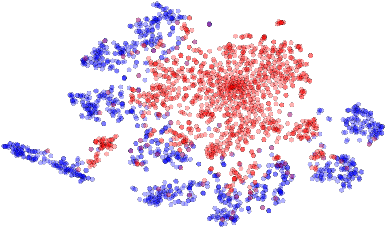
\includegraphics[width=0.45\textwidth]{./figures/adaptation_vis/pool2_mnist2inv_before.pdf}}\hfill%
  \subfigure[Adapted]{%%
    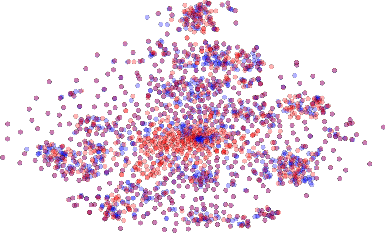
\includegraphics[width=0.45\textwidth]{./figures/adaptation_vis/pool2_mnist2inv_after.pdf}}%%
  \hspace*{\fill}%
  \end{minipage}%
  \begin{minipage}{.5\textwidth}
  \centering
  \small{{\sc Syn Numbers $ \rightarrow $ SVHN}: last hidden layer of the label predictor}
  \setcounter{subfigure}{0}
  \hspace*{\fill}%
  \subfigure[Non-adapted]{%%
    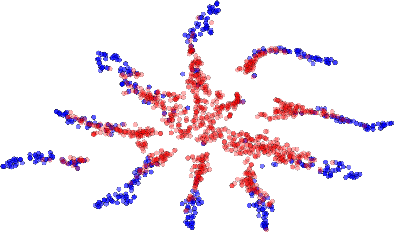
\includegraphics[width=0.45\textwidth]{./figures/adaptation_vis/before.pdf}}\hfill%
  \subfigure[Adapted]{%%
    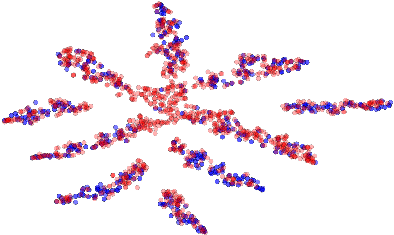
\includegraphics[width=0.45\textwidth]{./figures/adaptation_vis/after.pdf}}%%
  \hspace*{\fill}%
  \end{minipage}
  \caption{The effect of adaptation on the distribution of the extracted features (best viewed in color). The figure shows t-SNE \cite{Maaten13} visualizations of the CNN's activations {\bf (a)} in case when no adaptation was performed and {\bf (b)} in case when our adaptation procedure was incorporated into training. {\it Blue} points correspond to the source domain examples, while {\it red} ones correspond to the target domain. In all cases, the adaptation in our method makes the two distributions of features much closer.}
  \label{fig:exper_adapt_vis}
\end{figure*}

\subsection{Results}
\label{sect:exper_quant}

We now discuss the experimental settings and the results. In each case, we train on the source dataset and test on a different target domain dataset, with considerable shifts between domains (see \fig{exper_domains_examples}). The results are summarized in \tab{results} and \tab{results_office}. 

\vspace{2mm}\noindent {\bf MNIST $ \rightarrow $ MNIST-M.}
Our first experiment deals with the MNIST dataset~\cite{LeCun98} (source). In order to obtain the target domain ({\sc MNIST-M}) we blend digits from the original set over patches randomly extracted from color photos from BSDS500 \cite{Arbelaez11}. This operation is formally defined for two images $ I^{1}, I^{2} $ as $ I_{ijk}^{out} = | I_{ijk}^{1} - I_{ijk}^{2} | $, where $ i, j $ are the coordinates of a pixel and $ k $ is a channel index. In other words, an output sample is produced by taking a patch from a photo and inverting its pixels at positions corresponding to the pixels of a digit. For a human the classification task becomes only slightly harder compared to the original dataset (the digits are still clearly distinguishable) whereas for a CNN trained on MNIST this domain is quite distinct, as the background and the strokes are no longer constant. Consequently, the source-only model performs poorly. Our approach succeeded at aligning feature distributions (\fig{exper_adapt_vis}), which led to successful adaptation results (considering that the adaptation is unsupervised). At the same time, the improvement over source-only model achieved by subspace alignment (SA) \cite{Fernando13} is quite modest, thus highlighting the difficulty of the adaptation task. 

\vspace{2mm}\noindent {\bf Synthetic numbers $ \rightarrow $ SVHN.}
To address a common scenario of training on synthetic data and testing on  real data, we use Street-View House Number dataset {\sc SVHN} \cite{Netzer11} as the target domain and synthetic digits as the source. The latter ({\sc Syn ~Numbers}) consists of ~500,000 images generated by ourselves from Windows fonts by varying the text (that includes different one-, two-, and three-digit numbers), positioning, orientation, background and stroke colors, and the amount of blur. The degrees of variation were chosen manually to simulate SVHN, however the two datasets are still rather distinct, the biggest difference being the structured clutter in the background of SVHN images. 

The proposed backpropagation-based technique works well covering two thirds of the gap between training with source data only and training on target domain data with known target labels. In contrast, SA~\cite{Fernando13} does not result in any significant improvement in the classification accuracy, thus highlighting that the adaptation task is even more challenging than in the case of the MNIST experiment.

\vspace{2mm}\noindent {\bf MNIST $ \leftrightarrow $ SVHN.}
In this experiment, we further increase the gap between distributions, and test on {\sc MNIST} and {\sc SVHN}, which are significantly different in appearance. Training on SVHN even without adaptation is challenging --- classification error stays high during the first 150 epochs. In order to avoid ending up in a poor local minimum we, therefore, do not use learning rate annealing here. Obviously, the two directions ({\sc MNIST} $ \rightarrow $ {\sc SVHN} and {\sc SVHN} $ \rightarrow $ {\sc MNIST}) are not equally difficult. As {\sc SVHN} is more diverse, a model trained on SVHN is expected to be more generic and to perform reasonably on the MNIST dataset. This, indeed, turns out to be the case and is supported by the appearance of the feature distributions. We observe a quite strong separation between the domains when we feed them into the CNN trained solely on { \sc MNIST}, whereas for the {\sc SVHN}-trained network the features are much more intermixed. This difference probably explains why our method succeeded in improving the performance by adaptation in the {\sc SVHN} $ \rightarrow $ {\sc MNIST} scenario (see \tab{results}) but not in the opposite direction (SA is not able to perform adaptation in this case either). Unsupervised adaptation from MNIST to SVHN gives a failure example for our approach (we are unaware of any unsupervised DA methods capable of performing such adaptation).

\vspace{2mm}\noindent {\bf Synthetic Signs $ \rightarrow $ GTSRB.}
Overall, this setting is similar to the {\sc Syn Numbers} $ \rightarrow $ {\sc SVHN} experiment, except the distribution of the features is more complex due to the significantly larger number of classes (43 instead of 10). For the source domain we obtained~100,000 synthetic images (which we call {\sc Syn~Signs}) simulating various photoshooting conditions. Once again, our method achieves a sensible increase in performance once again proving its suitability for the synthetic-to-real data adaptation.

\begin{figure}
  \centering
  \setlength\figureheight{2.7cm}
  \setlength\figurewidth{6.8cm}
  % This file was created by matlab2tikz v0.5.0 running on MATLAB 8.3.
%Copyright (c) 2008--2014, Nico Schlömer <nico.schloemer@gmail.com>
%All rights reserved.
%Minimal pgfplots version: 1.3
%
%The latest updates can be retrieved from
%  http://www.mathworks.com/matlabcentral/fileexchange/22022-matlab2tikz
%where you can also make suggestions and rate matlab2tikz.
%
\begin{tikzpicture}[font=\scriptsize]

\begin{axis}[%
width=0.95092\figurewidth,
height=\figureheight,
at={(0\figurewidth,0\figureheight)},
scale only axis,
xmin=10000,
xmax=50000,
xlabel={Batches seen},
ymin=0,
ymax=1,
ylabel={Validation error},
axis x line*=bottom,
axis y line*=left,
legend style={at={($ (1,1) + (-0.1cm,-0.1cm) $)},anchor=north east,align=left,legend cell align=left,draw=black},
xmajorgrids,
ymajorgrids,
grid style={dashed}
]
\addplot [color=blue,solid,line width=1.0pt]
  table[row sep=crcr]{%
10500	0.199757996632997\\
11000	0.19162984006734\\
11500	0.190788089225589\\
12000	0.192918771043771\\
12500	0.196390993265993\\
13000	0.185527146464646\\
13500	0.190472432659933\\
14000	0.185606060606061\\
14500	0.183422769360269\\
15000	0.189051978114478\\
15500	0.191524621212121\\
16000	0.186079545454545\\
16500	0.179424452861953\\
17000	0.187684132996633\\
17500	0.187868265993266\\
18000	0.180923821548822\\
18500	0.187315867003367\\
19000	0.178661616161616\\
19500	0.18102904040404\\
20000	0.180555555555556\\
20500	0.176662457912458\\
21000	0.183791035353535\\
21500	0.179214015151515\\
22000	0.178898358585859\\
22500	0.178898358585859\\
23000	0.174479166666667\\
23500	0.174742213804714\\
24000	0.171059553872054\\
24500	0.177951388888889\\
25000	0.174794823232323\\
25500	0.174084595959596\\
26000	0.174636994949495\\
26500	0.169034090909091\\
27000	0.171191077441077\\
27500	0.170875420875421\\
28000	0.171506734006734\\
28500	0.170217803030303\\
29000	0.169244528619529\\
29500	0.169875841750842\\
30000	0.168744739057239\\
30500	0.17048085016835\\
31000	0.169454966329966\\
31500	0.167771464646465\\
32000	0.168849957912458\\
32500	0.168323863636364\\
33000	0.168718434343434\\
33500	0.165667087542088\\
34000	0.167376893939394\\
34500	0.169007786195286\\
35000	0.167140151515152\\
35500	0.165667087542088\\
36000	0.167850378787879\\
36500	0.169823232323232\\
37000	0.170691287878788\\
37500	0.16640361952862\\
38000	0.167981902356902\\
38500	0.169875841750842\\
39000	0.166771885521886\\
39500	0.169376052188552\\
40000	0.168087121212121\\
40500	0.165509259259259\\
41000	0.167718855218855\\
41500	0.168060816498317\\
42000	0.166035353535354\\
42500	0.166692971380471\\
43000	0.166429924242424\\
43500	0.167034932659933\\
44000	0.170349326599327\\
44500	0.169744318181818\\
45000	0.168218644781145\\
45500	0.166429924242424\\
46000	0.166324705387205\\
46500	0.168771043771044\\
47000	0.168034511784512\\
47500	0.168718434343434\\
48000	0.171059553872054\\
48500	0.170638678451178\\
49000	0.16819234006734\\
49500	0.168981481481481\\
50000	0.167902988215488\\
};
\addlegendentry{Real data only};

\addplot [color=cyan,solid,line width=1.0pt]
  table[row sep=crcr]{%
10500	0.9625\\
11000	0.79765625\\
11500	0.715625\\
12000	0.6140625\\
12500	0.52109375\\
13000	0.459375\\
13500	0.4484375\\
14000	0.421875\\
14500	0.39453125\\
15000	0.4109375\\
15500	0.34296875\\
16000	0.36875\\
16500	0.3359375\\
17000	0.36171875\\
17500	0.3171875\\
18000	0.3484375\\
18500	0.32421875\\
19000	0.315625\\
19500	0.346875\\
20000	0.31875\\
20500	0.35390625\\
21000	0.3265625\\
21500	0.33359375\\
22000	0.3171875\\
22500	0.28515625\\
23000	0.30546875\\
23500	0.309375\\
24000	0.2796875\\
24500	0.30859375\\
25000	0.30703125\\
25500	0.3078125\\
26000	0.28671875\\
26500	0.2875\\
27000	0.31484375\\
27500	0.2859375\\
28000	0.29375\\
28500	0.31328125\\
29000	0.3078125\\
29500	0.2859375\\
30000	0.2890625\\
30500	0.284375\\
31000	0.2953125\\
31500	0.26953125\\
32000	0.29921875\\
32500	0.30078125\\
33000	0.2640625\\
33500	0.309375\\
34000	0.2734375\\
34500	0.290625\\
35000	0.26796875\\
35500	0.3015625\\
36000	0.26796875\\
36500	0.2921875\\
37000	0.265625\\
37500	0.2765625\\
38000	0.2859375\\
38500	0.32109375\\
39000	0.28046875\\
39500	0.275\\
40000	0.24921875\\
40500	0.29140625\\
41000	0.26640625\\
41500	0.265625\\
42000	0.259375\\
42500	0.2765625\\
43000	0.26796875\\
43500	0.2765625\\
44000	0.27265625\\
44500	0.25546875\\
45000	0.26484375\\
45500	0.271875\\
46000	0.2703125\\
46500	0.26171875\\
47000	0.246875\\
47500	0.25078125\\
48000	0.29609375\\
48500	0.2640625\\
49000	0.26875\\
49500	0.26015625\\
50000	0.2578125\\
};
\addlegendentry{Synthetic data only};

\addplot [color=red,solid,line width=1.0pt]
  table[row sep=crcr]{%
10500	0.943892045454545\\
11000	0.943892045454545\\
11500	0.943892045454545\\
12000	0.943892045454545\\
12500	0.848300715488216\\
13000	0.658722643097643\\
13500	0.590593434343434\\
14000	0.475484006734007\\
14500	0.313946759259259\\
15000	0.235690235690236\\
15500	0.17879313973064\\
16000	0.152383207070707\\
16500	0.12912984006734\\
17000	0.114478114478114\\
17500	0.116214225589226\\
18000	0.1015625\\
18500	0.10066813973064\\
19000	0.101983375420875\\
19500	0.0914351851851852\\
20000	0.0895675505050505\\
20500	0.0894360269360269\\
21000	0.0827283249158249\\
21500	0.0798611111111111\\
22000	0.0859638047138047\\
22500	0.0799137205387205\\
23000	0.0778619528619529\\
23500	0.0737584175084175\\
24000	0.0742582070707071\\
24500	0.0776778198653199\\
25000	0.0771517255892256\\
25500	0.0725747053872054\\
26000	0.0739425505050505\\
26500	0.0734953703703704\\
27000	0.0730744949494949\\
27500	0.0688920454545455\\
28000	0.0702072811447811\\
28500	0.072337962962963\\
29000	0.0670244107744108\\
29500	0.0733638468013468\\
30000	0.0667613636363636\\
30500	0.0692340067340067\\
31000	0.0652093855218855\\
31500	0.0664720117845118\\
32000	0.0655776515151515\\
32500	0.0671296296296296\\
33000	0.0656039562289562\\
33500	0.0646043771043771\\
34000	0.0668665824915825\\
34500	0.0638678451178451\\
35000	0.065077861952862\\
35500	0.0649989478114478\\
36000	0.0672348484848485\\
36500	0.0668665824915825\\
37000	0.0626052188552189\\
37500	0.0652093855218855\\
38000	0.0626315235690236\\
38500	0.0627893518518518\\
39000	0.0613162878787879\\
39500	0.063236531986532\\
40000	0.0629208754208754\\
40500	0.0639467592592593\\
41000	0.0612899831649832\\
41500	0.0653409090909091\\
42000	0.0608691077441077\\
42500	0.0613425925925926\\
43000	0.0630260942760943\\
43500	0.060106271043771\\
44000	0.0638678451178451\\
44500	0.0602377946127946\\
45000	0.0577388468013468\\
45500	0.062684132996633\\
46000	0.0608164983164983\\
46500	0.0603167087542088\\
47000	0.0577651515151515\\
47500	0.0583175505050505\\
48000	0.0591329966329966\\
48500	0.0607112794612795\\
49000	0.0585805976430976\\
49500	0.0583175505050505\\
50000	0.0590540824915825\\
};
\addlegendentry{Both};

\end{axis}
\end{tikzpicture}%
  \caption{Semi-supervised domain adaptation for the traffic signs. As labeled target domain data are shown to the method, it achieves significantly lower error than the model trained on target domain data only or on source domain data only. \vspace{-4mm}}
  \label{fig:exper_semi_test}
\end{figure}

As an additional experiment, we also evaluate the proposed algorithm for semi-supervised domain adaptation, i.e.\ when one is additionally provided with a small amount of labeled target data. For that purpose we split {\sc GTSRB} into the train set (1280 random samples with labels) and the validation set (the rest of the dataset). The validation part is used solely for the evaluation and does not participate in the adaptation. The training procedure changes slightly as the label predictor is now exposed to the target data. \fig{exper_semi_test} shows the change of the validation error throughout the training. While the graph clearly suggests that our method can be used in the semi-supervised setting, thorough verification of semi-supervised setting is left for future work.


\vspace{2mm}\noindent {\bf Office dataset.} 
We finally evaluate our method on {\sc Office} dataset, which is a collection of three distinct domains: {\sc Amazon}, {\sc DSLR}, and {\sc Webcam}. Unlike previously discussed datasets, {\sc Office} is rather small-scale with only 2817 labeled images spread across 31 different categories in the largest domain. The amount of available data is crucial for a successful training of a deep model, hence we opted for the fine-tuning of the CNN pre-trained on the ImageNet \cite{Jia14} as it is done in some recent DA works \cite{Donahue14,Tzeng14,Hoffman14}. We make our approach more comparable with \cite{Tzeng14} by using exactly the same network architecture replacing domain mean-based regularization with the domain classifier.

Following most previous works, we evaluate our method using 5 random splits for each of the 3 transfer tasks commonly used for evaluation. Our training protocol is close to \cite{Tzeng14,Saenko10,Gong12} as we use the same number of labeled source-domain images per category. Unlike those works and similarly to e.g.\ DLID~\cite{Chopra13} we use the whole unlabeled target domain (as the premise of our method is the abundance of unlabeled data in the target domain). Under this transductive setting, our method is able to improve previously-reported state-of-the-art accuracy for unsupervised adaptation very considerably (\tab{results_office}), especially in the most challenging {\sc Amazon} $ \rightarrow $ {\sc Webcam} scenario (the two domains with the largest domain shift).

\section{VQA Dataset Analysis}
\label{sec:analysis}
%\vspace{\sectionReduceBot}
%%%%%%%%%%%%%%%%%%%%%%%%%%%%%%%%%%%%%%%%%%%%%%%%%%%%%%%%%%%
%%%%%%%%%%%%%%%%%%%%%%%%%%%%%%%%%%%%%%%%%%%%%%%%%%%%%%%%%%%
\begin{figure*}[t]
\centering
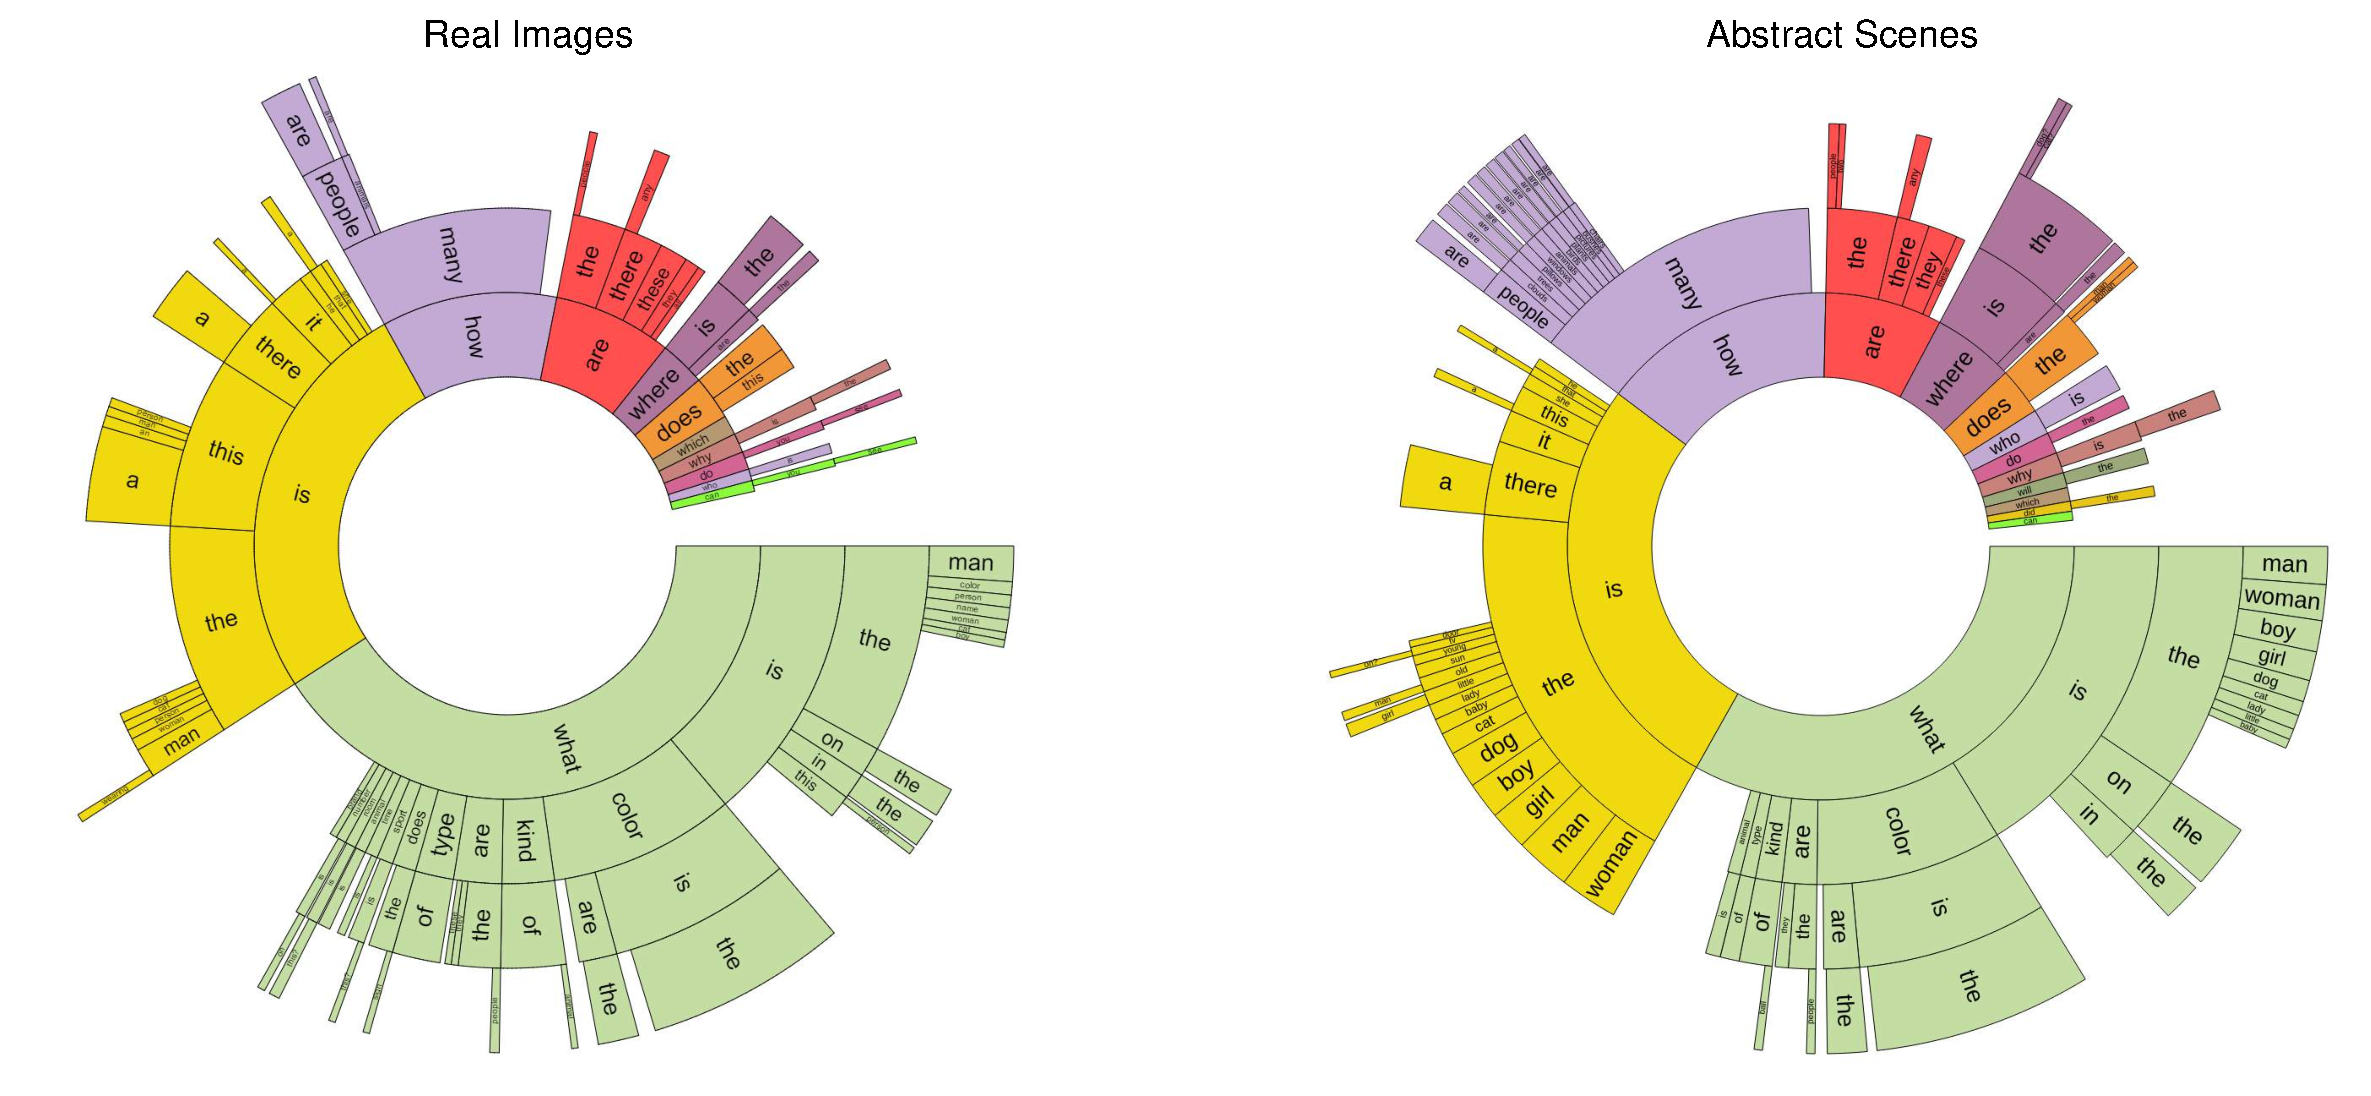
\includegraphics[width=1\linewidth]{figures/QuestionTypes3.pdf}
\caption{Distribution of questions by their first four words for a random sample of 60K questions for real images (left) and all questions for abstract scenes (right). The ordering of the words starts towards the center and radiates outwards. The arc length is proportional to the number of questions containing the word. White areas are words with contributions too small to show. }
%\vspace{-5pt}
\label{fig:QuesCluster}
%\setlength{\belowcaptionskip}{-10pt}
\end{figure*}
%%%%%%%%%%%%%%%%%%%%%%%%%%%%%%%%%%%%%%%%%%%%%%%%%%%%%%%%%%%

In this section, we provide an analysis of the questions and answers in the VQA train dataset.
To gain an understanding of the types of questions asked and answers provided, we visualize
the distribution of question types and answers. We also explore how often the questions may
be answered without the image using just commonsense information. Finally, we analyze whether
the information contained in an image caption is sufficient to answer the questions.

The dataset includes 614,163 questions 
%and a total of 
and 7,984,119 answers (including answers provided by workers with and without 
looking at the image) 
%and without looking at the image) 
for 204,721 images from the MS COCO dataset~\cite{coco} and 150,000 questions with 1,950,000 answers for $50,000$ abstract scenes.

%\textcolor{red}{
%We emphasize that the creation of a dataset of this scale and richness
%is a time consuming process, taking months to complete.
%While the entirety of the dataset has been collected,} at the time of original submission,
%120,520 questions with 270,210 answers for 50,000 MS COCO
%images and 30,000 questions with 79,740 answers for 10,000 abstract scenes had been collected.
%Please refer to the appendix for further details.
%\textcolor{red}{The results in this section still reflect that subset of the final dataset.}
%We emphasize that the creation of a dataset of this scale and richness
%is a time consuming process, taking months to complete.
%By our current estimates,
%approximately 5,000 questions and 40,000 answers are collected per day
%using Amazon Mechanical Turk (AMT).
%The entire dataset will take approximately three months to complete. At the time of submission,
%120,520 questions with 270,210 answers for 50,000 MS COCO
%images and 30,000 questions with 79,740 answers for 10,000 abstract scenes had been collected.
%Please refer to the appendix for further details.


%%%%%%%%%%%%%%%%%%%%%%%%%%%%%%%%%%%%%%%%%%%%%%%%%%%%%%%%%%%
%\vspace{\subsectionReduceTop}
\subsection{Questions}
%\vspace{\subsectionReduceBot}
%%%%%%%%%%%%%%%%%%%%%%%%%%%%%%%%%%%%%%%%%%%%%%%%%%%%%%%%%%%

\textbf{Types of Question.}
Given the structure of questions generated in the English language,
we can cluster questions into different types based on the words that start the question.
\figref{fig:QuesCluster} shows the distribution of questions based on the first four
words of the questions for both the real images (left) and abstract scenes (right).
Interestingly, the distribution of questions is quite similar for both real images and abstract scenes.
This helps demonstrate that the type of questions elicited by the abstract scenes is similar to
those elicited by the real images. There exists a surprising variety of question types,
including ``What is$\ldots$'', ``Is there$\ldots$'', ``How many$\ldots$'', and ``Does the$\ldots$''.
Quantitatively, the percentage of questions for different types is shown in \tableref{tab:typeacc}. Several example questions and answers are shown in \figref{fig:qualResults}.
%\textbf{Sub-Types.}
A particularly interesting type of question is the ``What is$\ldots$'' questions, since they have a
diverse set of possible answers. See the appendix for visualizations for ``What is$\ldots$'' questions.

\textbf{Lengths.}
\figref{fig:QuesLen} shows the distribution of question lengths.
We see that most questions range from four to ten words.


\begin{comment}\begin{table}[h]
{\small
\begin{tabular}{@{\extracolsep{\fill}}p{2cm}|ccccc@{\extracolsep{\fill}}}
%\toprule
Dataset  & Yes & No\\
%\midrule
Real   & 18.21 & 14.06 \\
Abstract & 26.54 & 16.70 \\
\end{tabular}
}
\vspace{5pt}
\caption{Percentage of ``yes'' and ``no'' questions in the real and abstract datasets.}
\label{table:yesno}
%\vspace{\captionReduceBot}
\end{table}
\end{comment}

%%%%%%%%%%%%%%%%%%%%%%%%%%%%%%%%%%%%%%%%%%%%%%%%%%%%%%%%%%%
\begin{figure}[t]
\centering
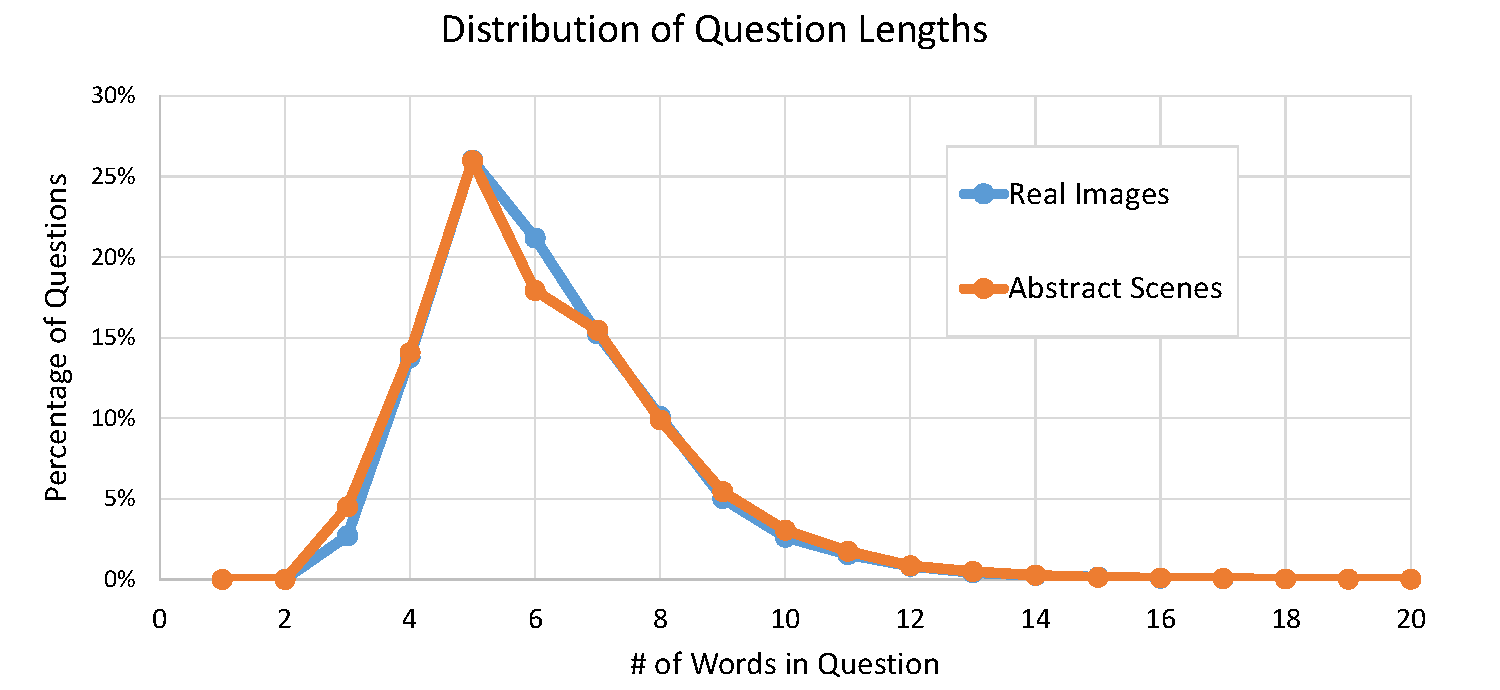
\includegraphics[width=1\linewidth]{figures/Lengths.pdf}
%\vspace{-9pt}
\caption{Percentage of questions with different word lengths for real images and abstract scenes.}
%\vspace{-5pt}
\label{fig:QuesLen}
%\setlength{\belowcaptionskip}{-10pt}
\end{figure}
%%%%%%%%%%%%%%%%%%%%%%%%%%%%%%%%%%%%%%%%%%%%%%%%%%%%%%%%%%%




\begin{figure*}
\centering
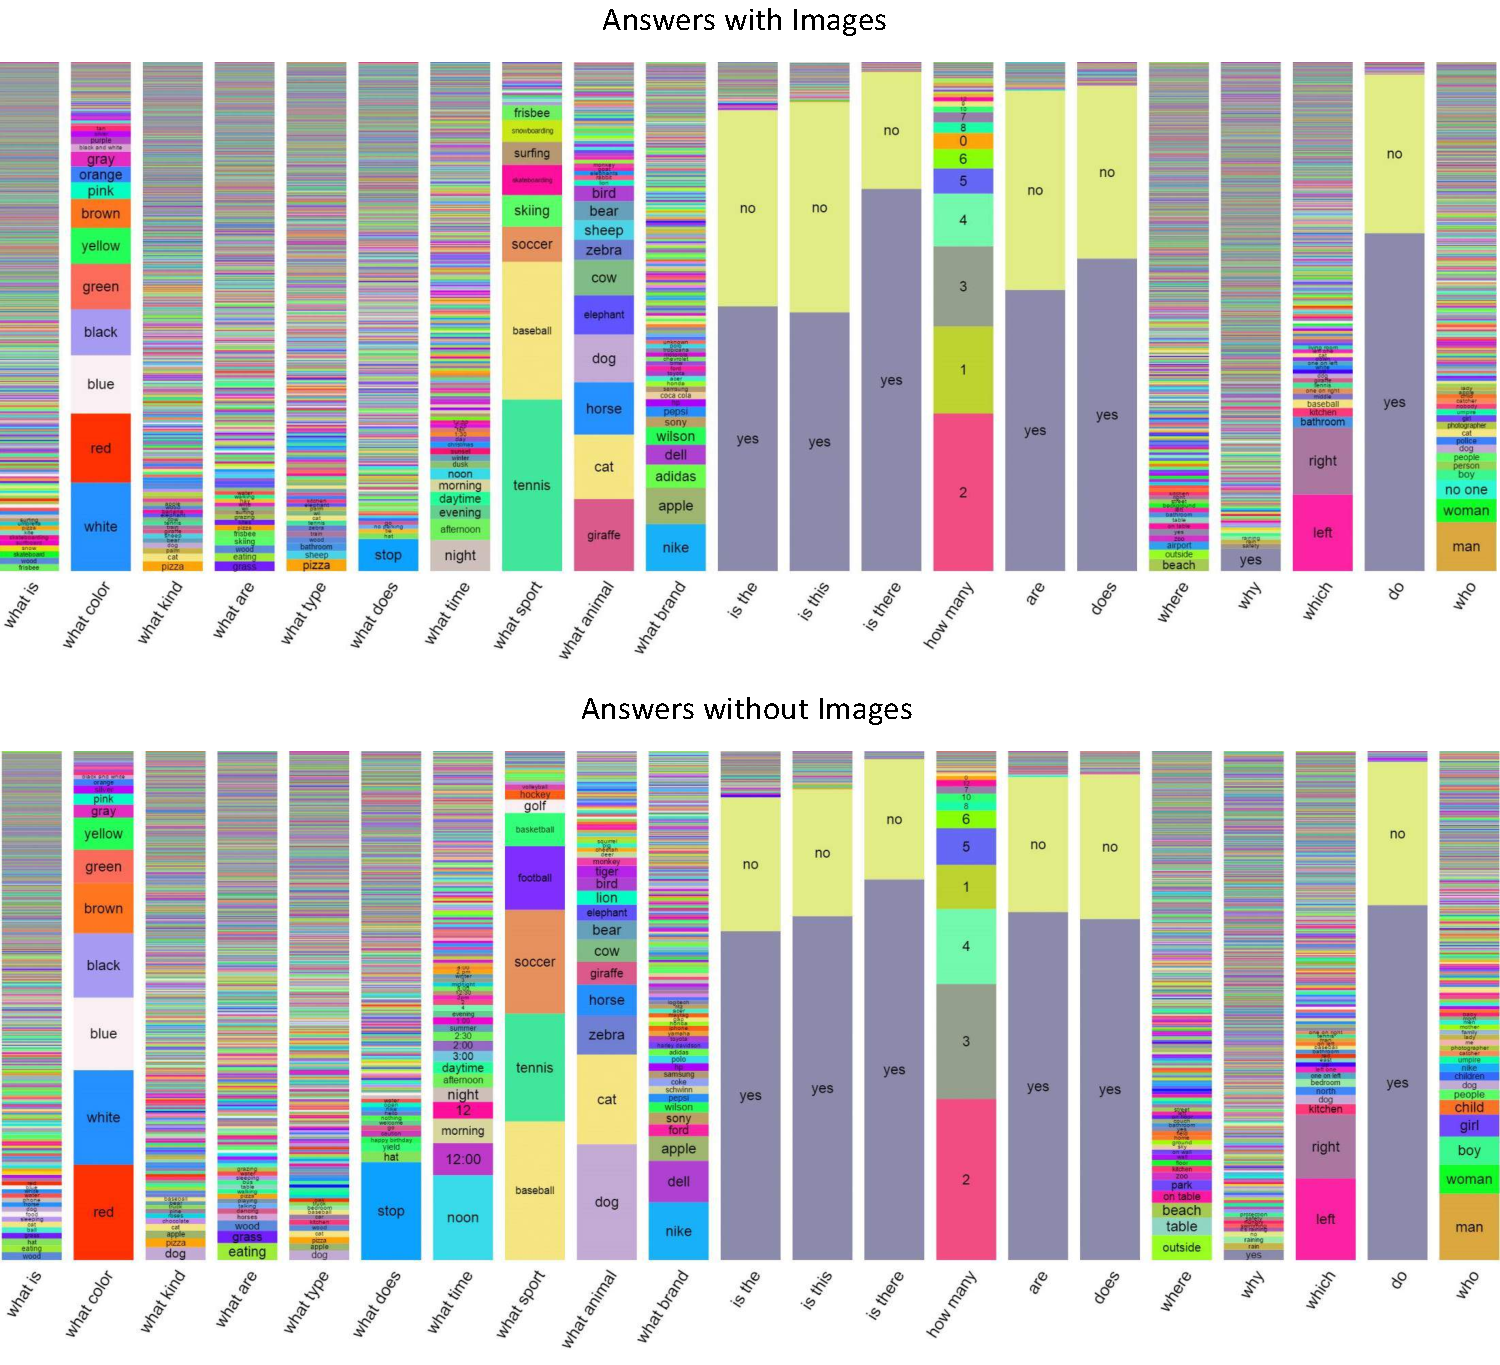
\includegraphics[width=1\linewidth]{figures/answers.pdf}
%\vspace{-5pt}
\caption{Distribution of answers per question type for a random sample of 60K questions for real images when subjects provide answers when given the image (top) and when not given the image (bottom).}
%\vspace{-5pt}
\label{fig:AnsPerQues}
%\setlength{\belowcaptionskip}{-10pt}
\end{figure*}


%%%%%%%%%%%%%%%%%%%%%%%%%%%%%%%%%%%%%%%%%%%%%%%%%%%%%%%%%%%
%\vspace{\subsectionReduceTop}
\subsection{Answers}
%\vspace{\subsectionReduceBot}
%%%%%%%%%%%%%%%%%%%%%%%%%%%%%%%%%%%%%%%%%%%%%%%%%%%%%%%%%%%

%\textbf{Typical Answers for Different Question Types.}
\textbf{Typical Answers.}
%Next, we analyze the answers provided for different question types.
\figref{fig:AnsPerQues} (top) shows the distribution of answers for several question types.
We can see that a number of question types, such as ``Is the\ldots'', ``Are\ldots'', and ``Does\ldots'' are
typically answered using ``yes'' and ``no'' as answers.
%\textcolor{red}{Question types such as ``How many\ldots'' are answered using numbers. $12.31\%$ and $14.48\%$ of the questions are answered using numbers on real images and abstract scenes, respectively.}
Other questions such as ``What is\ldots'' and ``What type\ldots'' have a rich diversity
of responses. Other question types such as ``What color\ldots'' or ``Which\ldots'' have more specialized responses,
such as colors, or ``left'' and ``right''. 
See the appendix for a list of the most popular answers.

\textbf{Lengths.}
Most answers consist of a single word, with the distribution of answers containing one, two, or three words, respectively being $89.32\%$, $6.91\%$, and $2.74\%$ for real images and $90.51\%$, $5.89\%$, and $2.49\%$ for abstract scenes.
%$89.16\%$, $7.00\%$, and $2.77\%$ of answers containing one, two, or three words, respectively.
The brevity of answers is not surprising, since the questions tend to elicit specific
information from the images. This is in contrast with image captions that generically
describe the entire image and hence tend to be longer. The brevity of our answers makes
automatic evaluation feasible. While it may be tempting to believe the brevity of the answers
makes the problem easier, recall that they are human-provided open-ended answers to
open-ended questions. The questions typically require complex reasoning to arrive at these
deceptively simple answers (see \figref{fig:qualResults}).
There are currently 23,234 unique one-word answers in our dataset for real images and 3,770 for abstract scenes.
%There are currently 10,011 unique one-word answers in our dataset.

\textbf{`Yes/No' and `Number' Answers.}
Many questions are answered using either ``yes'' or ``no'' (or sometimes ``maybe'') -- 
$38.37\%$ and $40.66\%$ of the questions on real images and abstract scenes respectively. 
Among these `yes/no' questions, there is a bias towards %answering with 
``yes'' -- %with ``yes'' being preferred %$61.32\%$ and $58.46\%$ 
$58.83\%$ and $55.86\%$ of `yes/no' answers are ``yes'' for real images and abstract scenes. 
Question types such as ``How many\ldots'' are answered using numbers -- 
$12.31\%$ and $14.48\%$ of the questions on real images and abstract scenes are `number' questions. 
``2'' is the most popular answer among the `number' questions, making up 
$26.04\%$ of the `number' answers for real images and $39.85\%$ for abstract scenes. 

\textbf{Subject Confidence.}
When the subjects answered the questions, we asked
``Do you think you were able to answer the question correctly?''.
\figref{fig:ConfScores} shows the distribution of responses. A majority of the answers
were labeled as confident for both real images and abstract scenes. % respectively.

\textbf{Inter-human Agreement.}
Does the self-judgment of confidence correspond to the answer agreement between subjects?
\figref{fig:ConfScores} shows the percentage of questions in which 
(i) $7$ or more, 
(ii) $3-7$, or 
(iii) less than $3$ subjects agree on the answers given their average confidence score 
(0 = not confident, 1 = confident).
As expected, the agreement between subjects increases with confidence.
However, even if all of the subjects are confident the answers may still vary.
This is not surprising since some answers may vary, yet have very similar meaning, such as ``happy'' and ``joyful''.

\begin{figure}[t]
\centering
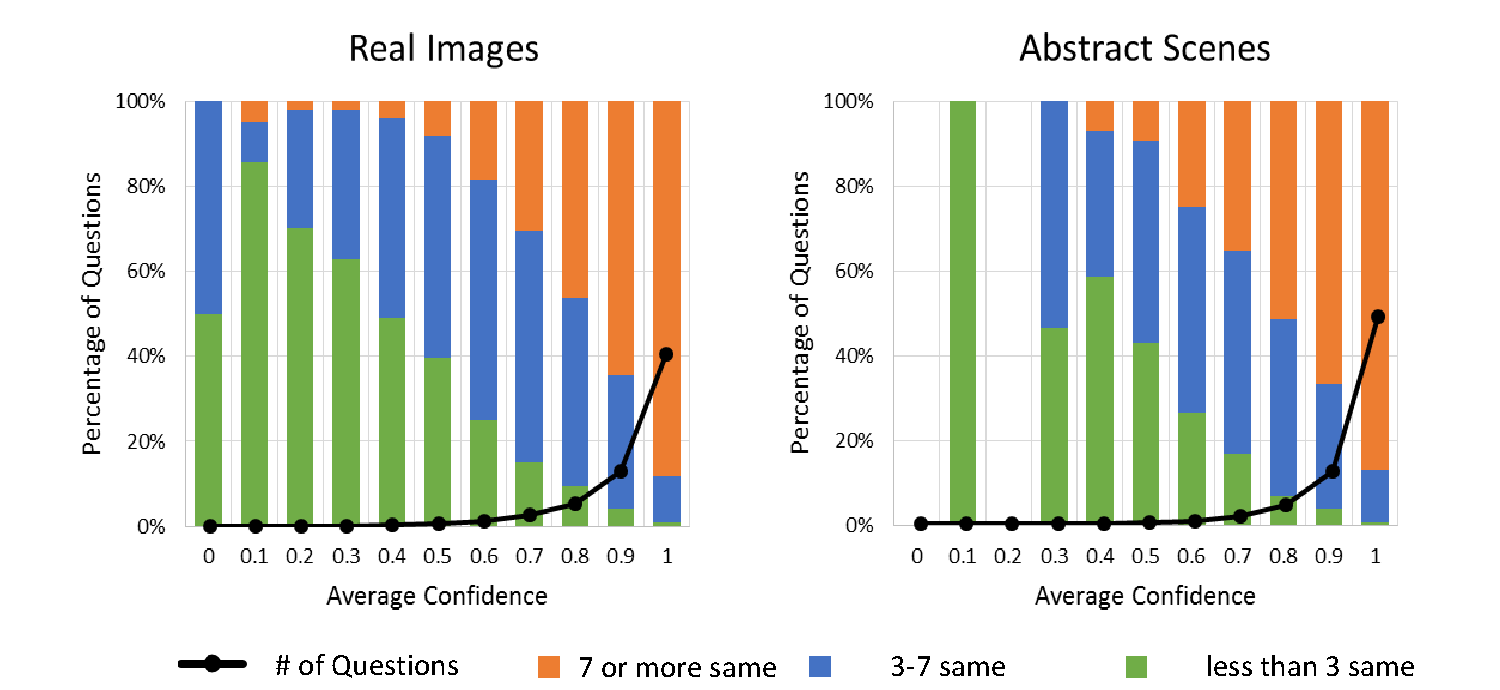
\includegraphics[width=1\linewidth]{figures/Confidence.pdf}
%\vspace{-5pt}
\caption{Number of questions per average confidence score (0 = not confident, 1 = confident) for real images and abstract scenes (black lines). Percentage of questions where 7 or more answers are same, 3-7 are same, less than 3 are same (color bars). }
%\vspace{-7pt}
\label{fig:ConfScores}
%\setlength{\belowcaptionskip}{-10pt}
\end{figure}

As shown in \tableref{table:commonsense_acc} (Question + Image), there is significant inter-human
agreement in the answers for both real images ($83.30\%$) and abstract scenes ($87.49\%$). 
%when humans are provided both the question and image while answering the question.
Note that on average each question has $2.70$ unique answers for real images and $2.39$ for abstract scenes. 
The agreement is significantly higher ($>95\%$) for \quotes{yes/no} questions and lower for other questions ($<76\%$), possibly due to the fact that we perform exact string matching and do not account for synonyms, plurality, \etc. Note that the automatic determination of synonyms is a difficult problem, since the level of answer granularity can vary across questions.




%%%%%%%%%%%%%%%%%%%%%%%%%%%%%%%%%%%%%%%%%%%%%%%%%%%%%%%%%%%
%\vspace{\subsectionReduceTop}
\subsection{Commonsense Knowledge}
\label{sec:cs}
%\vspace{\subsectionReduceBot}
%%%%%%%%%%%%%%%%%%%%%%%%%%%%%%%%%%%%%%%%%%%%%%%%%%%%%%%%%%%
\begin{figure*}[t]
 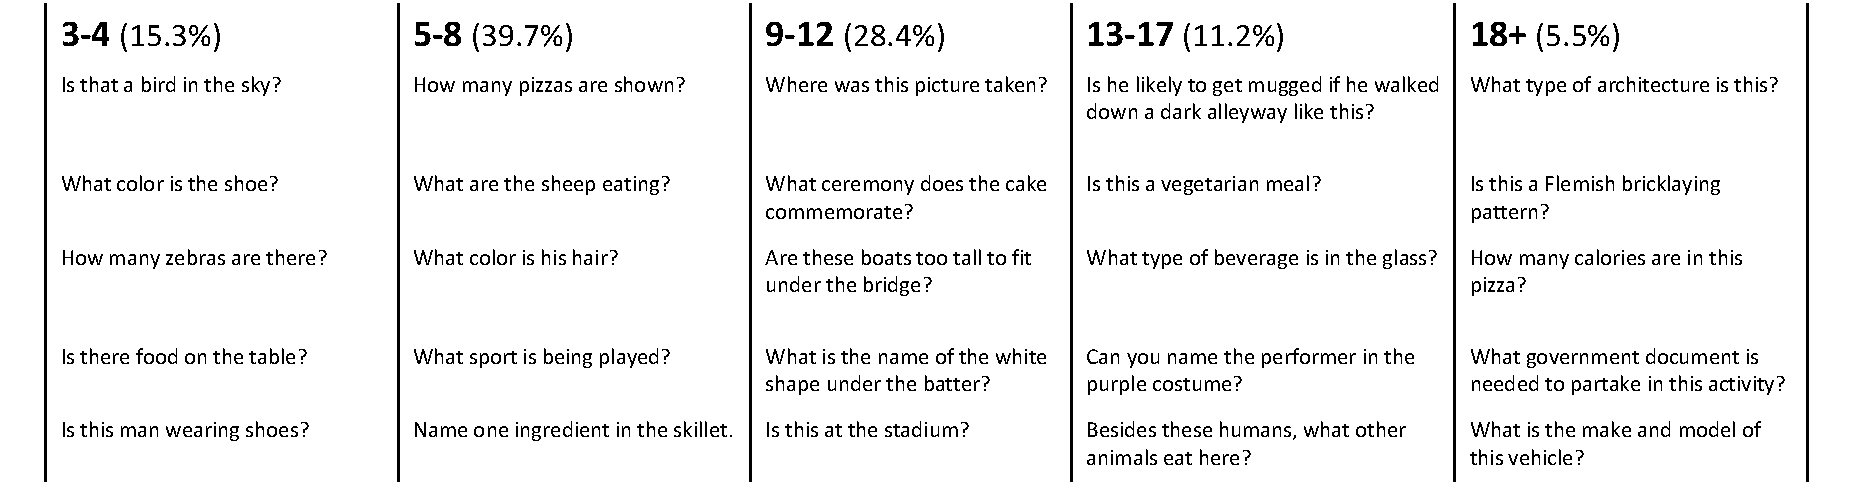
\includegraphics[width=\linewidth]{figures/age.pdf}
 \centering
\caption{\small Example questions judged by Mturk workers to be answerable by different age groups. The percentage of questions falling into each age group is shown in parentheses.}
 \label{fig:age}
 \end{figure*}
 	
\textbf{Is the Image Necessary?}
%Can the questions be answered using commonsense knowledge alone without the need for an image,
%\eg, ``What is the color of the sheep?''?
Clearly, some questions can sometimes be
answered correctly using commonsense knowledge alone without the need for an image,
\eg, ``What is the color of the fire hydrant?''.
We explore this issue by asking three subjects to answer
the questions \emph{without seeing the image} (see the examples in blue in \figref{fig:qualResults}).
In \tableref{table:commonsense_acc} (Question), we show the percentage of questions for which
the correct answer is provided over all questions, ``yes/no'' questions, and the other questions that
are not ``yes/no''. For ``yes/no'' questions, the human subjects respond better than chance.
For other questions, humans are only correct about $21\%$ of the time. This demonstrates that
understanding the visual information is critical to VQA and that commonsense information alone is not sufficient.

To show the qualitative difference in answers provided with and without images,
we show the distribution of answers for various question types in \figref{fig:AnsPerQues} (bottom).
The distribution of colors, numbers, and even ``yes/no'' responses is surprisingly different for answers
with and without images.
 
\textbf{Which Questions Require Common Sense?}
In order to identify questions that require commonsense reasoning to answer, we conducted 
two AMT studies (on a subset 10K questions from the real images of VQA trainval) asking subjects --
\begin{compactenum} 
\item Whether or not they believed a question required commonsense to answer the question, and 
\item The youngest age group that they believe a person must be in order to be able to correctly answer the question -- 
toddler (3-4), 
younger child (5-8), 
older child (9-12), 
teenager (13-17), 
adult (18+).
\end{compactenum}
Each question was shown to 10 subjects. We found that 
for $47.43\%$ of questions 3 or more subjects voted `yes' to commonsense, 
($18.14\%$: 6 or more).  
In the `perceived human age required to answer question' study, we found the following distribution of responses: 
toddler: $15.3\%$,
younger child: $39.7\%$, 
older child: $28.4\%$, 
teenager: $11.2\%$, 
adult: $5.5\%$.
In Figure \ref{fig:age} we show several questions for which a majority of subjects picked the specified age range. Surprisingly the perceived age needed to answer the questions is fairly well distributed across the different age ranges. As expected the questions that were judged answerable by an adult (18+) generally need specialized knowledge, whereas those answerable by a toddler (3-4) are more generic.
 
We measure the degree of commonsense required to answer a question as the percentage of subjects (out of 10) who voted ``yes'' in our ``whether or not a question requires commonsense'' study.
A fine-grained breakdown of average age and average degree of common sense (on a scale of $0-100$) required to answer a question is shown in \tableref{tab:typeacc}. The average age and the average degree of commonsense across all questions is $8.92$ and $31.01\%$ respectively. 

%\arxiv{To compute average age and average degree of commonsense across questions, we first compute the average age and average degree of commonsense (binary response scaled to $0-100$) per question (by taking average across 10 subjects for each question) and then take average across questions.} 

It is important to distinguish between:
\begin{compactenum}
\item How old someone needs to be to be able to answer a question correctly,  and
\item How old people \emph{think} someone needs to be to be able to answer a question correctly. 
\end{compactenum}

Our age annotations capture the latter -- perceptions of MTurk workers in an uncontrolled environment. As such, the relative ordering of question types in \tableref{tab:typeacc} is more important than absolute age numbers.
%The relative ordering of question types is more important than the absolute age numbers. It is important to note that the age annotations we have collected are just perceived ages: how old people -- untrained MTurk workers in an uncontrolled environment -- \emph{think} someone needs to be to be able to answer a question correctly.}
The two rankings of questions in terms of common sense required according to the two studies 
were largely correlated (Pearson's rank correlation: 0.58). 

%%%%%%%%%%%%%%%%%%%%%%%%%%%%%%%%%%%%%%%%%%%%%%%%%%%%%%%%%%%
\begin{table}[t]
\setlength{\tabcolsep}{3.2pt}
{\small
\begin{center}
%\begin{tabular}{@{}llccc@{}}
%\toprule
%Dataset & Input & All & Yes/No & Other \\
%%\hline
%\midrule
%    & Question & 40.81 & 67.60 & 21.22 \\
%Real   & Question + Caption* & 57.47 & 78.97 & 44.41 \\
%    & Question + Image & 83.30 & 95.77 & 72.67 \\
%%\hline
%\midrule
% & Question & 43.27 & 66.65 &  23.66 \\
%Abstract & Question + Caption* & 54.34 & 74.70 & 40.18 \\
% & Question + Image & 87.49 & 95.96 & 75.33 \\
%\bottomrule
%\end{tabular}
\begin{tabular}{@{}llcccc@{}}
\toprule
Dataset & Input & All & Yes/No & Number & Other \\
%\hline
\midrule
    & Question & 40.81 & 67.60 & 25.77 & 21.22 \\
Real   & Question + Caption* & 57.47 & 78.97 & 39.68 & 44.41 \\
    & Question + Image & 83.30 & 95.77 & 83.39 & 72.67 \\
%\hline
\midrule
 & Question & 43.27 & 66.65 & 28.52 & 23.66 \\
Abstract & Question + Caption* & 54.34 & 74.70 & 41.19 & 40.18 \\
 & Question + Image & 87.49 & 95.96 & 95.04 & 75.33 \\
\bottomrule
\end{tabular}
\end{center}
}
%\vspace{-7pt}
\caption {Test-standard accuracy of human subjects when asked to answer the 
question without seeing the image (Question), 
seeing just a caption of the image and not the image itself (Question + Caption), 
and seeing the image (Question + Image). 
Results are shown for all questions, ``yes/no'' \& ``number'' questions, and other questions 
that are neither answered ``yes/no'' nor number. 
All answers are free-form and not multiple-choice. 
*\hspace{1pt}These accuracies are evaluated on a subset of 3K train questions (1K images).}
% \textcolor{red}{and are not directly comparable to the corresponding numbers in older version.}}
\label{table:commonsense_acc}
%\vspace{\captionReduceBot}
%\vspace{-5pt}
\end{table}
%%%%%%%%%%%%%%%%%%%%%%%%%%%%%%%%%%%%%%%%%%%%%%%%%%%%%%%%%%%


%%%%%%%%%%%%%%%%%%%%%%%%%%%%%%%%%%%%%%%%%%%%%%%%%%%%%%%%%%%
%\vspace{\subsectionReduceTop}
\subsection{Captions \textbf{\vs} Questions}
%\vspace{\subsectionReduceBot}
%%%%%%%%%%%%%%%%%%%%%%%%%%%%%%%%%%%%%%%%%%%%%%%%%%%%%%%%%%%


Do generic image captions provide enough information to answer the questions?
\tableref{table:commonsense_acc} (Question + Caption) shows the percentage of questions answered
correctly when human subjects are given the question and a human-provided caption
describing the image, but not the image. As expected, the results are better than when humans are shown the questions alone.
However, the accuracies are significantly lower than when subjects are shown the actual image.
This demonstrates that in order to answer the questions correctly, deeper image understanding 
(beyond what image captions typically capture) is necessary. In fact, we find that the distributions of nouns, verbs, and adjectives mentioned in captions is statistically significantly different from those mentioned in our questions + answers (Kolmogorov-Smirnov test, $p<.001$) for both real images and abstract scenes. See the appendix for details. 
%This motivates the VQA task as a way to learn further information about visual scenes.

\label{sec:conclusion}
We introduce a novel neural network architecture, the Synchronized Spectral CNN (SyncSpecCNN), for semantic annotation on 3D shape graphs. To share coefficients and conduct multi-scale analysis in different parts of a single shape graph, we introduce a spectral parametrization of dilated convolutional kernels. To allow parameter sharing across related but different shapes that may be represented by very different graphs, we introduce a spectral transformer network to synchronize different spectral domains. The effectiveness of different components in our network is validated through extensive experiments. Jointly these contributions lead to state-of-the-art performance on various semantic annotation tasks including 3D shape part segmentation and 3D keypoint prediction.

%\section*{Acknowledgments}
%Suppressed for review.
%{\small 
%We thank Kyunghyun Cho for his easy-to-understand neural machine translation code and Alexander Rush for providing us %with the test data and for helping us make as fair a comparison as possible with their system.
%}
%\pagebreak
% include your own bib file like this:
%\bibliographystyle{acl}
%\bibliography{acl2016}
\bibliography{summarization}
\bibliographystyle{acl2016}

\end{document}
